\documentclass[aps,
%twocolumn,
superscriptaddress,notitlepage]{revtex4-1}
\usepackage{graphicx}
\usepackage{bm}
\usepackage{amsmath}
\usepackage{amsfonts}
\usepackage{amssymb}
\usepackage{array}
\usepackage{xcolor}
\usepackage{dcolumn}
\usepackage{longtable}
\usepackage{hyperref}
\usepackage{natbib}
\usepackage{stmaryrd}%
\usepackage{color}
\usepackage{wasysym} % for hexagon and star of david in equation
\usepackage{siunitx}
\usepackage{enumitem}
\usepackage{lipsum}
\usepackage{amsmath,amsthm}
\usepackage{amsfonts}
\usepackage{amssymb}
\usepackage{bbold}
\usepackage{amssymb}
\usepackage{epstopdf}
\usepackage{times}
\usepackage{mathrsfs}
\usepackage{color}
\usepackage{gensymb}
\usepackage{times}
\usepackage{subfigure}
\usepackage[]{graphicx}
\usepackage{amssymb}
\usepackage{amsmath}
\usepackage{bm}
\usepackage{bm,amsmath}

\definecolor{mygreen}{RGB}{98,174,37}
\definecolor{myred}{RGB}{211,0,45}
\definecolor{myblue}{RGB}{0,126,148}

%\usepackage[utf8x]{inputenc}
%\bibliographystyle{plain}
%\bibliographystyle{unsrtnat}
%\usepackage[square,sort,comma,numbers]{natbib}
%\usepackage{amsmath,amsfonts, amsthm, amssymb}
%\usepackage{newlfont}
%\usepackage{fancyhdr}
%\usepackage[Glenn]{fncychap}
%\usepackage{fullpage}

%\usepackage[T1]{fontenc}
%\usepackage{array,multicol}
%\thispagestyle{empty}
%\usepackage[pdftex]{graphicx}
%%\usepackage{graphicx,xcolor}
%\usepackage{framed}
%\usepackage{setspace}
%\usepackage{listings}
%\usepackage{tikz}
%\usepackage{pgfplots}
%\usepackage{tikz-3dplot}
%\usepackage{booktabs}
%\usepackage{bm}
%\usepackage{siunitx}

%\tdplotsetmaincoords{70}{150}
%\pgfplotsset{compat=newest}

%\usepackage{setspace} % Espaciado entre lineas
%%\onehalfspacing
%\setstretch{1.3}
% general defs
\def\ep{\varepsilon}
\def\eps{\varepsilon}
\def\half{\frac{1}{2}}
\def\phi{\varphi}
\def\RR{\mathbb R}
\def\NN{\mathbb N}
\def\supp{{\rm supp}}
\def\di{\displaystyle}
\def\ri{\rightarrow}
\def\calx{{\cal X}}
\def\intom{\int_\Omega}
\def\huo{H^1_0(\Omega )}
\def\incep{\left\{\begin{array}{ll} }
 \def\termin{\end{array}\right. }
\def\intga{\int_\Gamma}
\def\wik{\widetilde{K}}
\def\wie{\widetilde{E}}
%\def\uu{[ u]}
\def\vu{[ v-u]}
\def\la2{\lambda^2}
\def\proof{{\it Proof.}\ }
\def\endproof{\nolinebreak\hfill\rule{2mm}{2mm}}
\def\rh{\rightharpoonup}
\def\dst{\displaystyle}
\newcommand{\bs}{{\boldsymbol \sigma}}
\newcommand{\bss}{{\boldsymbol s}}
\newcommand{\bep}{{\boldsymbol \varepsilon}}
\newcommand{\bt}{{\boldsymbol \tau}}
\newcommand{\btt}{{\boldsymbol t}}
\newcommand{\bnu}{{\boldsymbol \nu}}
\newcommand{\bu}{{\boldsymbol u}}
\newcommand{\bmm}{{\boldsymbol m}}
\newcommand{\br}{{\boldsymbol r}}
\newcommand{\bR}{{\boldsymbol R}}
\newcommand{\be}{{\boldsymbol e}}
\newcommand{\bc}{{\boldsymbol c}}
\newcommand{\bv}{{\boldsymbol v}}
\newcommand{\bg}{{\boldsymbol \gamma}}
\newcommand{\bF}{{\boldsymbol F}}
\newcommand{\bK}{{\boldsymbol K}}
\newcommand{\bV}{{\boldsymbol V}}
%\newcommand{\bni}{{\boldsymbol n}}
\newcommand{\bn}{{\boldsymbol e}_3}
\newcommand{\nn}{{\boldsymbol e}_3}
\newcommand{\bal}{{\boldsymbol \alpha}}
\newcommand{\bff}{{\boldsymbol f}}
\newcommand{\ba}{{\boldsymbol a}}
\newcommand{\bb}{{\boldsymbol b}}
\newcommand{\bx}{{\boldsymbol x}}
\newcommand{\U}{{\cal U}}
\newcommand{\T}{{\cal T}}
\newcommand{\F}{{\cal F}}
\newcommand{\E}{{\cal E}}
\newcommand{\LL}{{\cal L}}
\newcommand{\N}{{\cal N}}
\newcommand{\K}{{\cal K}}
\newcommand{\W}{{\cal W}}
%\newcommand{\bN}{\boldsymbol {\cal N}}
\newcommand{\bN}{\boldsymbol  N}
\newcommand{\bDD}{\boldsymbol  D}
\newcommand{\bM}{\boldsymbol  M}
\newcommand{\bE}{{\boldsymbol  E}}
\newcommand{\bA}{\boldsymbol {\cal A}}
\newcommand{\bU}{\boldsymbol {\cal U}}
\newcommand{\bCC}{\boldsymbol {\cal C}}
\newcommand{\bMM}{\boldsymbol {\cal M}}
\newcommand{\bAA}{{\boldsymbol A}}
\newcommand{\bphi}{{\boldsymbol \phi}}
\newcommand{\bPsi}{{\boldsymbol \Psi}}
\newcommand{\bPi}{{\boldsymbol \Pi}}

\newcommand{\bni}{{\boldsymbol n}}
\newcommand{\bI}{{\boldsymbol I}}
\newcommand{\bS}{{\boldsymbol S}}
\newcommand{\D}{ {\cal D}}
\newcommand{\Oo}{ {\cal O}}
\newcommand{\oo}{{ {\mathcal o}}}

\def\R{\mathbb{R}}
\newcommand{\I}{{\boldsymbol {\cal I}}}
\newcommand{\bT}{{\boldsymbol {\cal T}}}
\newcommand{\bTT}{{\boldsymbol T}}
\newcommand{\bD}{{\boldsymbol{\cal D}}}
\newcommand{\bSS}{{\boldsymbol{\cal S}}}
%%%%%%%%%%%%%%%%%%%%%%
\newcommand{\C}{{\mathbb{C}}}         % \C for C (complex numbers)
\newcommand{\Q}{{\mathbb{Q}}}         % \Q for Q (rational numbers)
%\newcommand{\R}{{\mathbb{R}}}         % \R for R (real numbers)
\newcommand{\Z}{{\mathbb{Z}}}         % \Z for Z (integers)
%\newcommand{\N}{{\mathbb{N}}}         % \N for N (natural numbers)


\newcommand\DD{\mathcal{D}}
%\newcommand\T{\mathcal{T}}
%\newcommand\nn{\boldsymbol{n}}
\newcommand\uu{\boldsymbol{u}}
\newcommand\vv{\boldsymbol{v}}
\newcommand\bC{\boldsymbol{C}}
%\newcommand\bb{\boldsymbol{b}}
\newcommand\VV{\boldsymbol{V}}
\newcommand\UU{\boldsymbol{U}}
\newcommand\SSS{\boldsymbol{S}}
\newcommand\sig{\boldsymbol{\sigma}}
\newcommand\vep{\boldsymbol{\varepsilon}}
\newcommand\val{\boldsymbol{\alpha}}
\newcommand\vtau{\boldsymbol{\tau}}
\newcommand\vphi{\boldsymbol{\phi}}
\newcommand\bpsi{\boldsymbol{\psi}}

\newcommand\bd{\boldsymbol{d}}
\newcommand\bgg{\boldsymbol{g}}

\newcommand\nor{\boldsymbol{n}}
\newcommand\ee{\boldsymbol{e}}
\newcommand\brX{\bar{X}}


%\newtheorem{thm}{Theorem}[section]
%\newtheorem{lem}[thm]{Lemma}
%\newtheorem{prop}[thm]{Proposition}
%\newtheorem{cor}[thm]{Corollary}
%\newtheorem{rem}[thm]{Remark}  %remarca numerotata
%\newtheorem{prop1}[thm]{}
%\newtheorem{defn}[thm]{Definition}
%\newtheorem{defi}[thm]{Definition}
%\newtheorem*{remark}{Remark} %remarca nenumerotata
%\renewcommand{\theequation}{\arabic{equation}}
%
%\newtheorem{definition}[thm]{Definition}
%\newtheorem{proposition}[thm]{Proposition}
%\numberwithin{equation}{section}

%\usepackage{lineno}
%\linenumbers
%\modulolinenumbers[1]
%\usepackage{marginnote}


%\usepackage{hyperref}
%\hypersetup{
%  colorlinks   = true,    % Colours links instead of ugly boxes
%  urlcolor     = blue,    % Colour for external hyperlinks
%  linkcolor    = blue,    % Colour of internal links
%  citecolor    = blue     % Colour of citations
%}
%%%%%%%%%%%%%%%%%%%%%%%%%

\begin{document}
%\title{An accurate computation of true stress in compression experiments in the presence of localized deformation}

%\title{Self-induced  marginality in plastically deformed crystals}
%\title{Two-stage yielding   of pristine crystals}
\title{Amorphous crystals}
\author{O.U. Salman}
\affiliation{
LSPM, CNRS UPR3407, Université Sorbonne Paris Nord, 93400, Villateneuse, France}
%\affiliation{
%Lund University, Department of Mechanical Engineering Sciences, Lund, Sweden}
%\author{G. Tejedor}
%\affiliation{
%LSPM, CNRS UPR3407, Université Sorbonne Paris Nord, 93400, Villateneuse, France}
%\author{A. Ahadi}
%\affiliation{
%Lund University, Department of Mechanical Engineering Sciences, Lund, Sweden}
%\author{Nikolai  Gorbushin}
%\affiliation{
%LSPM, CNRS UPR3407, Université Sorbonne Paris Nord, 93400, Villateneuse, France}
%\affiliation{
%PMMH, CNRS UMR 7636 ESPCI ParisTech, 10 Rue Vauquelin, 75005, Paris, France}
\author{N. Gorbushin}
\affiliation{
PMMH, CNRS UMR 7636 ESPCI PSL, 10 Rue Vauquelin, 75005, Paris, France}
\author{ L. Truskinovsky}
\affiliation{
PMMH, CNRS UMR 7636 ESPCI PSL, 10 Rue Vauquelin, 75005, Paris, France}

\date{\today}
\begin{abstract}
Quasi-brittle yielding is a salient feature  of well-annealed glassy materials. Here we show that almost the same phenomenon characterizes plastic yielding in  model 2D perfect crystals. 
In such systems the elastic stage of deformation terminates  with a nonlinear elastic instability resulting in massive nucleation of dislocations.  As we show this system spanning (first) yield type event  effectively converts the atomic configuration from  crystalline  to a glassy. The subsequent deformation closely resembles quasi-brittle yielding of the ensuing  pseudo-amorphous system. To corroborate these claims we present a detailed study of  dislocation dynamics  in  a    prototypical square crystal  subjected to quasistatic loading. Our main tool is a novel mesoscopic tensorial model  (MTM) of crystal plasticity representing a conceptual trade-off between continuum  and atomic descriptions. In addition to overall strain response,  the MTM approach allows one  to  capture  intermittent statistics of dislocational avalanches. In close parallel  to what is known about plasticity of glassy systems, here  we also discover that both pre- and post- (second) yield  avalanches in emerging 'amorphous crystal' exhibit power law statistics with  matching exponents indicating marginal stability of the associated defect configurations. 
\end{abstract}
\maketitle
\noindent

 \section{Introduction}
Despite intense focus on the subject  in the last years, the phenomenon of  \emph{plastic yield} in  crystalline  solids  remains rather mysterious~\cite{Zaiser2006-gk,jian2024prediction,ortiz1999plastic,Papanikolaou2017-ld,kosterlitz2016kosterlitz,khantha1997mechanism,hochrainer2014continuum,langer2019statistical,Derlet2016-mp,ispanovity2010submicron}.
 It can be characterized as a  more or less abrupt loss of elastic rigidity and it also marks a transition from largely reversible to strongly irreversible deformation. For a  crystal  subjected to quasi-static loading in a hard device an intriguing   related question is why the memory of  local atomic neighborhoods, ensuring elastic or quasi-elastic response,  suddenly deteriorates allowing  the system  to abruptly sever a  link with its deformation history.  An even more challenging  question  concerns the nature of post-yield plastic flow which often exhibits  intermittent fluctuations and shows  scale free spatial organization.The goal of the present paper is to  address these questions in a  narrow but  fundamental setting  of  quasi-brittle  plastic yielding of  pristine (perfect,  defect free) crystals~\cite{Sethna2017,ghimenti2024shear,Salman2021,perchikov2024,Baggio2023,Baggio2023-qu,Zhang2020-ax}. 
The peculiarity of this particular setting  is related to the fact that, rather surprisingly,  very similar quasi-brittle  plastic yielding  is  also a salient feature  of some  glassy materials which lack any crystal symmetry and are structurally indistinguishable from liquids~\cite{kamani2024brittle,berthier2024yielding,Shang2020,shang2024yielding,singh2020brittle,richard2021brittle,pollard2022yielding,Lin2014-bx,parisi2017shear,derlet2021micro}.

To build a conceptual bridge  between plasticity of crystals and glasses,  we  show that plastic yielding in stylized 2D  pristine crystals can be represented as a two-stage process.  During the first stage of the yielding,  massive dislocation nucleation results in the formation of what is effectively a glassy dislocational configuration, see also  \cite{Lehtinen2016-qy,Sethna2017,Ovaska2017}.
 The ensued plastic flow  can be  viewed as largely 'caged'  which implies  non-collective  spatially localized dislocation rearrangements.  The second stage of the yielding interrupts this  flow abruptly through a system size, catastrophic  dislocational avalanche. It is this stage  that is  very similar to quasi-brittle yielding  in amorphous plasticity as it likewise  reveals itself through the   formation of  system-size  shear bands. In both crystals and glasses the subsequent plastic flow is stationary with stress reaching a characteristic plateau. It remains to be said that the discussed behavior concerns model crystals with suppressed hardening. More specifically, 
 to corroborate our claims we present a detailed study of  dislocation dynamics  in  a prototypical  square crystal  subjected to non-generic quasistatic loading by shear strain applied  along one of two the slip directions. Our main tool is a novel mesoscopic tensorial model  (MTM) of crystal plasticity representing a conceptual trade-off between continuum  and atomic descriptions~\cite{Salman2011,Salman2012b,Baggio2019,Salman2021,perchikov2024,Baggio2023,Baggio2023-qu,Zhang2020-ax}.


In view of the implied crystal-glass analogy, we begin by mentioning  some facts about quasi-brittle plastic yield  in glassy amorphous systems.  It is known that  under quasi-static  strain control, such systems exhibit  initially an almost reversible nominally-elastic  response even though  the overall stress increase  is   occasionally interrupted  by small stress drops revealing highly localized quasi-plastic rearrangements.   At a  critical  strain  such  response  gives way to fully global  plastic deformation  leading to stress  saturation.  In this stationary regime, short elastic stages coexist with  stress drops caused by localized  plastic shear transformations which occasionally  also induce long-range system-spanning rearrangements.  The transition to this constant-stress regime, which  is the one usually  interpreted as plastic yielding, can be of two types.  In ductile yielding we observe  a continuous crossover towards a stress plateau with only small stress overshoot which can be stretched over a large strain range.  In contrast, quasi-brittle yielding involves catastrophic failure through the sudden formation of system-spanning localized shear bands.   It was shown  that ductile  yielding takes place in  rapidly quenched glasses with  higher  degree of disorder while quasi-brittle yielding  is characteristic for more structured  highly annealed glass samples.  In the case of glasses,  such bi-modal yielding behavior  was successfully  reproduced numerically  using  prototypical elasto-plastic models in which  individual  linear elastic elements  could yield above some critical stress   triggering similar instabilities in other elements \cite{Nicolas2018-iy,Rodney2011-ld,popovic2018elastoplastic,Tanguy2021-ap,TALAMALI2012275}. 
Some theoretical approaches have also been advanced to supported these empirical findings \cite{Parley2024-jb,karmakar2010statistical,ozawa2018random,Divoux2024-ks}. 


  
As we have already mentioned, the main goal of the present  paper is to  extend the obtained  understanding of quasi-brittle yielding from amorphous  to crystal plasticity.  The two phenomena are sometimes perceived as fundamentally different in view of the observation that dislocations, the main carriers of plastic deformations  crystals, are absent in amorphous solids. However, the elementary mechanical events  behind the propagation  of individual dislocations  and behind the local advance of amorphous plasticity by  shear transformation zones, are basically the same and can be in both cases described  as  triggering of Eshelby-type shear eigenstrains \cite{Picard2004,Budrikis2017-ex,Cai2006-fe}.
Moreover, behind both amorphous and crystal plasticity is the evolution of elastic incompatibility which can be  characterized in both cases by elastic curvature induced by the associated metric tensor \cite{Moshe2015-rm,Baggioli2022-nx,Bowick2009-bl,Katanaev1992-kl,Sozio2020-tg}. 

In building a connection between crystalline and amorphous plasticity,  the  first challenge is to choose a relevant modeling framework which would   describe  adequately  crystal dislocations while being still compatible with the  modeling language  of  amorphous plasticity.  It is clear that engineering crystal plasticity, which  is  formulated within classical continuum framework  and relies on macroscale phenomenological constitutive relations, is not appropriate for this purpose since even dislocation cores there are not resolved. Numerous computational alternatives to continuum plasticity have been developed ranging from molecular dynamics (MD) \cite{Arsenlis2007-oz,Zepeda-Ruiz2021-bm,Ponga2020-kd,Lafourcade2025-pc} and similarly microscopic phase-field crystal method (PFC) \cite{Chan2010-qt,Salvalaglio2020-aw,Zhong2025-df} to the more coarse-grained phase field dislocation dynamics (PFDD), \cite{Javanbakht2016-dr,Beyerlein2016-av,Koslowski2002-dn,Wang:2003zh},  discrete dislocation dynamics (DDD), \cite{Devincre2008-mw,Ispanovity2014-ra,Gomez-Garcia2006-zn,Po2014-qu,Lu2022-ai,Bertin2024-jw,Nasir-Tak2025-kq} and, continuum dislocation dynamics (CDD) \cite{Starkey2020-yv,Zhang2025-cm,Acharya2022-ur,Acharya2006-du}. 
The multi-scale quasi-continuum model (QC) \cite{Rodney1999-em,Van-Koten2011-tt,Miller2002-pa,Zhang2018-in}. 
attempted to bridge all the scales while fully comprehensibly accounting for each of them. A detailed discussions of strengths and shortcomings of all these approaches can be found in \cite{Salman2021,perchikov2024,Baggio2023-qu}. 

They were all successful in addressing particular time and length scales, with higher-scale models (more coarse-grained) relying on input from lower-scale models (less coarse-grained). However,  the ability of the existing approaches to capture the correct statistics of plastic fluctuations, while also accounting for large lattice rotations and adequately representing the crystallographic nature of lattice-invariant shears, remains rather limited \cite{Weiss2021-tt,Weiss2015-eh}



To deal with these important aspects of crystal plasticity we rely in this paper on a more recent  Landau-inspired  MTM  approach   representing a conceptual trade-off between continuum  and atomic descriptions It can deal adequately with dislocation cores  while operating with engineering concepts of stress and strain\cite{Ericksen1970,ericksen1973loading,Ericksen1977,Ericksen1980,ericksen1989weak,parry1976elasticity,Parry1977,Parry1998,Folkins1991,Conti2004-sv,Salman2011,Salman2012b,Baggio2019,Salman2021,perchikov2024,Baggio2023,Baggio2023-qu,Zhang2020-ax}.

It can be viewed as an extension of the local QC model or as a tensorial version of the PFDD, accounting geometrically adequately for both large strains and large rotations. MTM describes faithfully short-range interactions between dislocations and  can deal with  anisotropic nonlinear elasticity. Moreover,  it resolves in continuum setting the full crystallographic symmetry, including lattice-invariant shears \cite{Engel1986-tm,Michel2001,schwarzenberger1972classification,Bhattacharya2004,pitteri2002continuum} .

 Behind the emergence of the continuum stresses and strains in MTM lies the spatial averaging over a mesoscopic length scale: the latter characterizes the size of a maximal cluster of atoms which can be assumed to deform homogeneously. The MTM belongs to the class of mesoscopic elasto-plastic  models  used in the studies of amorphous plasticity, but instead of using conventional Eshelby elastic propagator,  it deals directly with geometrically and physically nonlinear  elasticity of inhomogeneous solid bodies and instead of simplified description of plastic slip, it accounts adequately for crystallographically specific lattice invariant shears.  The resulting approach  has the advantage over DDD of describing without any special phenomenological assumptions, the  topological changes in dislocation configurations such as nucleation, annihilation and  interaction with obstacles, all  in a self-consistent manner and only relying on the  assumptions about the  inter-atomic potential. Most importantly, it allows one to resolve  scale-free dislocational avalanches, responsible for intermittent fluctuations accompanying steady plastic flows in low symmetry crystals.  We mention that various other  MTM-related  approaches have been also explored  in the literature  \cite{Denoual2010,Gao2019,Gao2020,Gao2020a,Gao2020f,Gao2020c,Biscari2015-ci,Arbib2020,Arbib2023,Arbib2025}.


In our study of the phenomenon of quasi-brittle yielding of pristine model crystals,  we use  the most simple but still  non-trivial   setting. Specifically, to simulate athermal quasistatic loading of perfect square crystals in simple shear, we use the 2D  MTM approach, which is thoroughly reviewed   to make the presentation fully self contained. As we have already mentioned, our main finding is the two stage structure of plastic yielding.
The   first stage is a nonlinear elastic instability of a homogeneous crystal which involves dramatic  proliferation of dislocations  and effectively transforms an ideal crystal into a quasi-amorphous solid. The subsequent deformation of such 'primed' crystal is strongly reminiscent of quasi-brittle plastic yield of a well annealed glass. It involves a 'microplasticity'  stage which ends abruptly with a formation of  system spanning grain boundaries. The corresponding post-(second)yield plastic deformation closely resembles  amorphous plastic flow which is sometimes interpreted as a regime of extended criticality.  It is marked by the formation of a stress plateau and involves intermittent  avalanche type rearrangements of  dislocational patterns which can be both local and global.  In parallel, to what is known about plasticity of glassy systems, here  we also discover that both pre- and post-(second) yield  avalanches exhibit power law statistics with matching exponents indicative of  marginal stability. 

The rest of the paper is organized as follows. In Section 2 we review  the main concepts of the MTM approach. The macroscopic results of our numerical experiments are summarized in Section 3. Statistical analysis of fluctuations is presented in Section 4. The last Section 5 contains our conclusions and indicates some open problems.


\section{The model}


In overview, the MTM is a  geometrically nonlinear theory of Landau-type where the role of the order parameter  is played by the
metric tensor (characterizing local deformation). In the corresponding 2D continuum theory the elastic energy  density is assumed to respect the full $GL(2, \mathbb{Z})$ symmetry of a Bravais lattices represented by 3x3 invertible matrices $\bf m$ with integer entries and unit determinants. This implies that such energy density is a multi-well function of tensorial parameter with  the bottoms of the energy wells corresponding to lattice invariant deformations. In the numerical implementation of the MTM, the space of admissible deformations is reduced to compatible piece-wise-affine mappings. Therefore, the outcome of the   numerical energy
minimization depends on the value of the internal length   representing the size of the mesoscopic finite element which  brings a cut-off scale into the theory. Given the large magnitude of the associated
transformation strains, different phases end up being localized at the scale of mesoscopic elements, and the domain boundaries appear macroscopically as linear defects  representing mesoscopic dislocations. 

\begin{figure}[ht!]
\centering
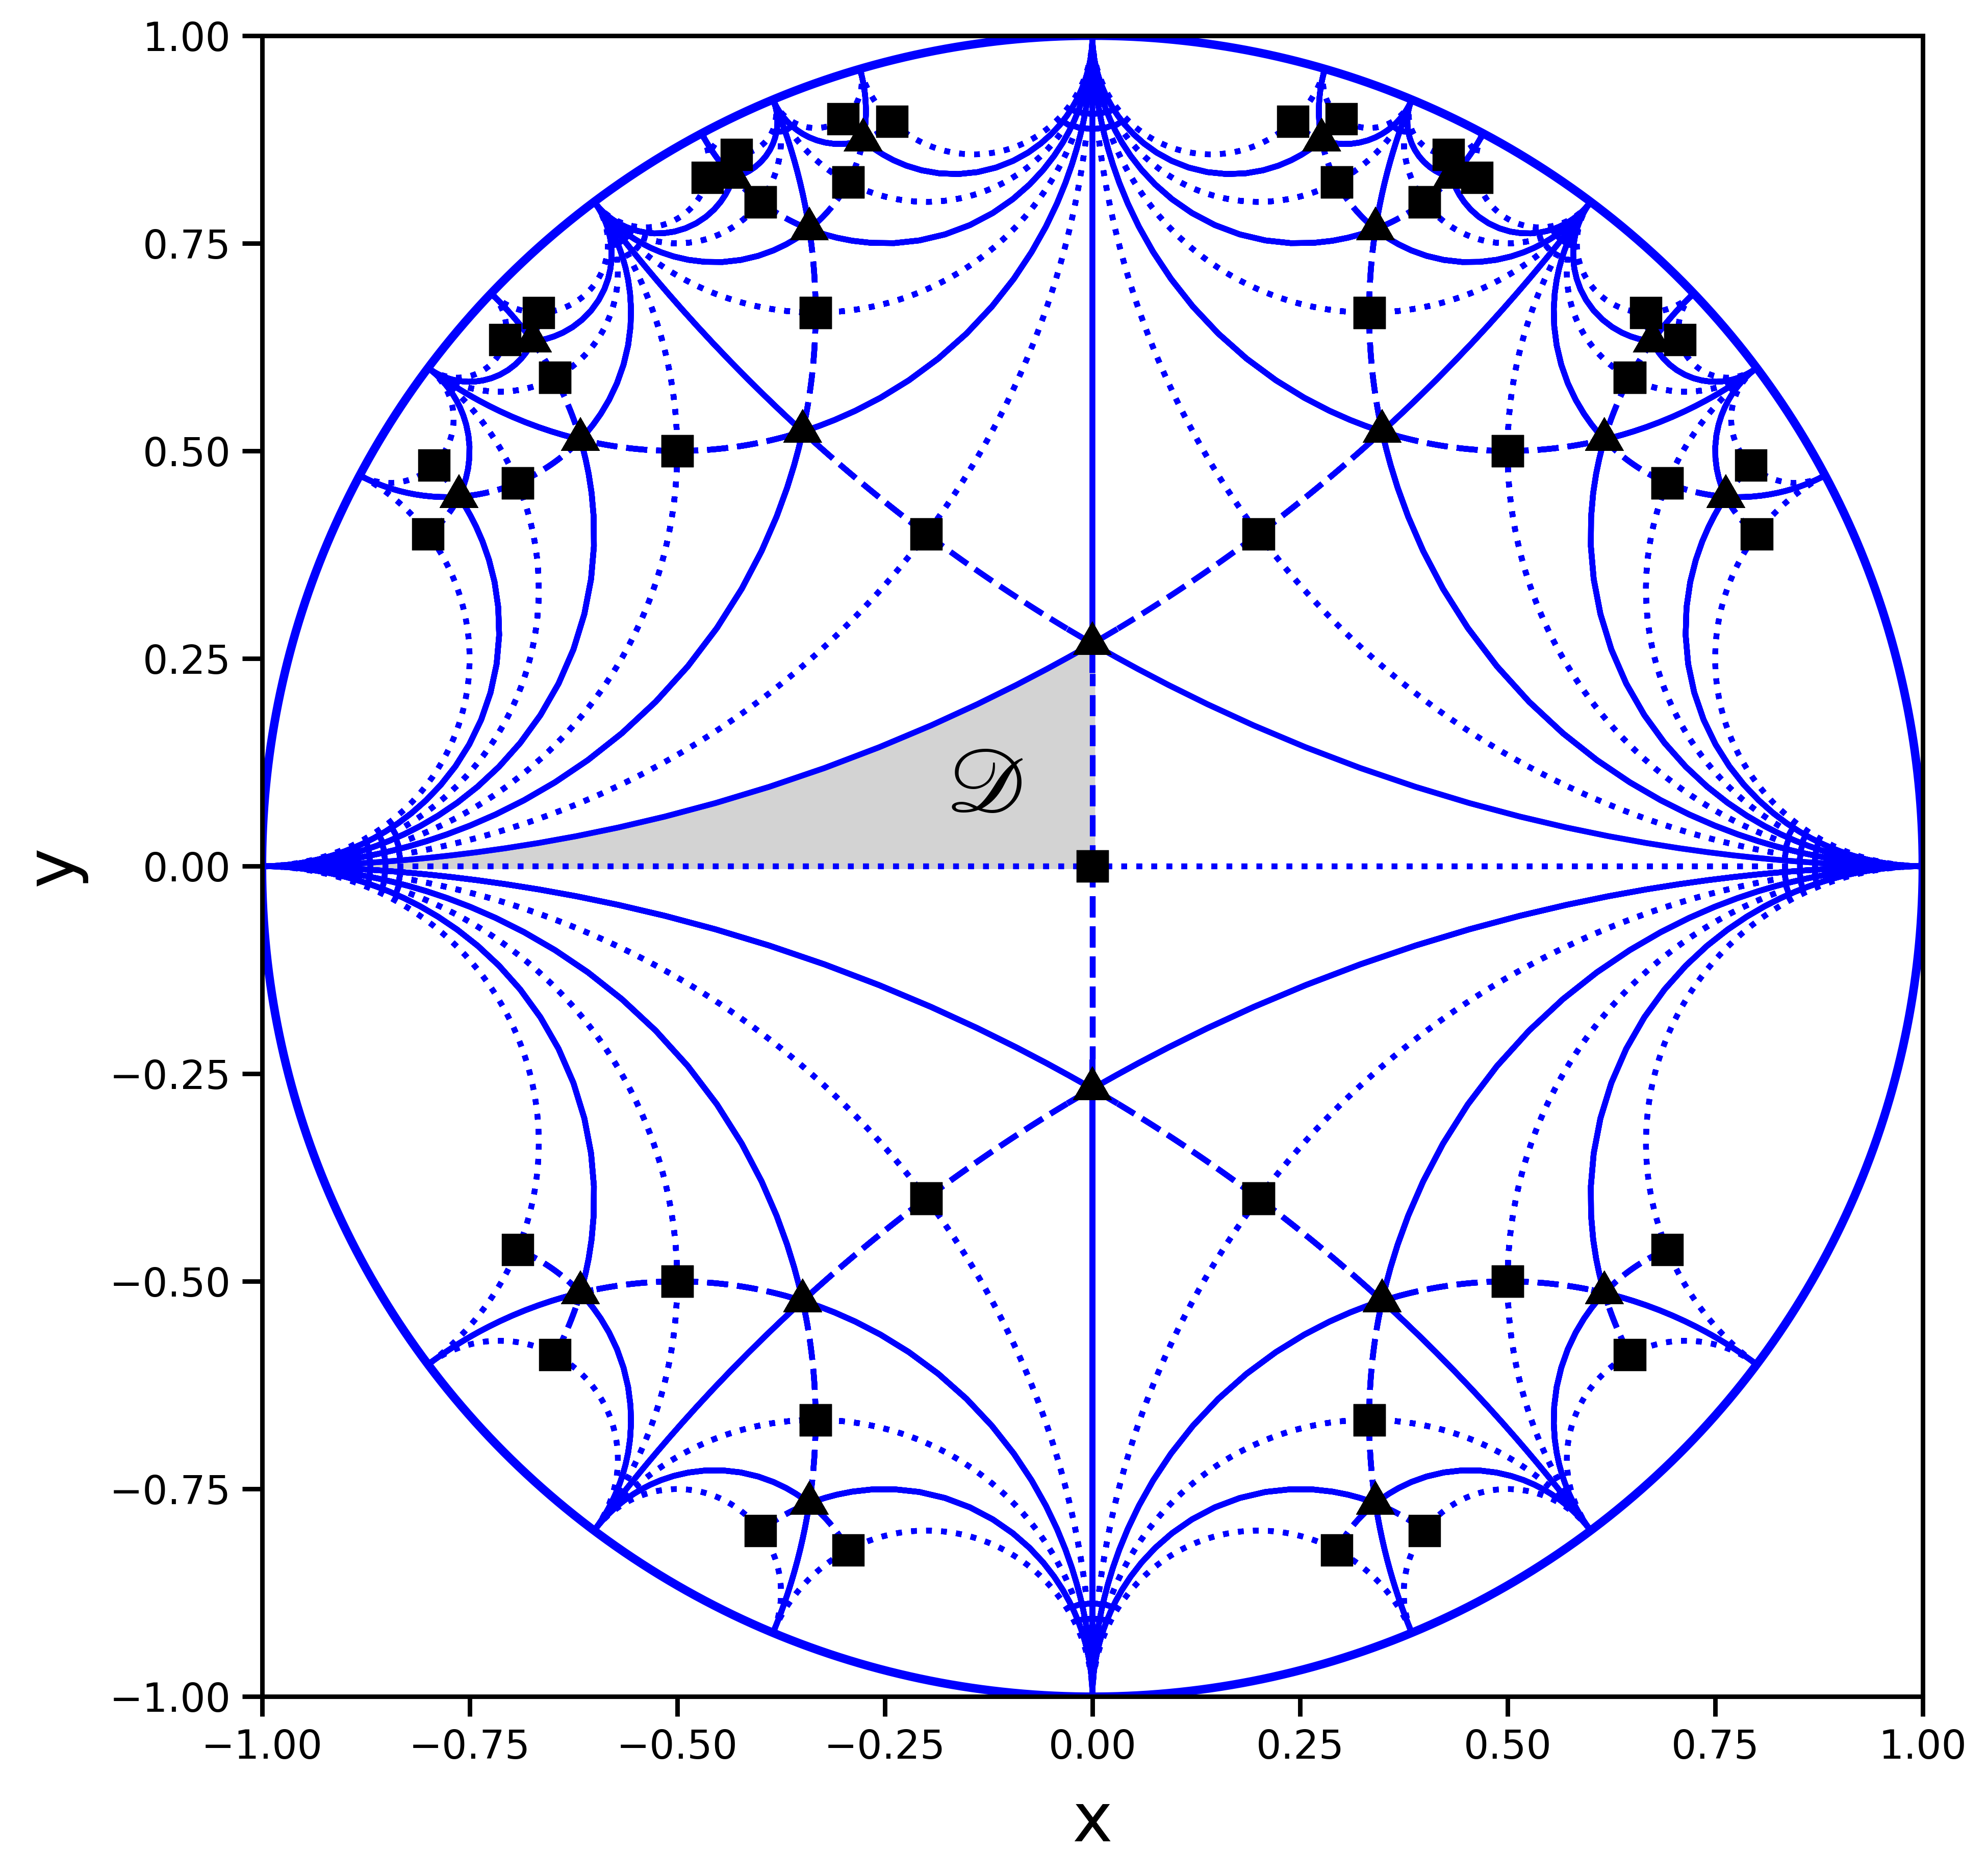
\includegraphics[scale=0.8]{figures_ordering/figure_01.png}
\caption{Tessellation of the metric tensor configurational space into fundamental periodicity domains using Poincaré disk coordinates. The tessellation consists of $GL(2, \mathbb{Z})$ copies of the fundamental domain highlighted in gray. Black squares and triangles denote regions corresponding to high-symmetry square and triangular lattice bases.}
\label{fig:atlas0}
\end{figure}



\subsection{Elastic energy}

In the 2D version of the MTM approach the configurational space of metric tensors is tessellated into an infinite number of equivalent domains, where equivalence is understood in terms of the symmetry transformations induced by   the infinite group $GL(2, \mathbb{Z})$.  If the the energy density  is known in one of such tensorial periodicity domains, it can be extended to the whole configurational space.   To be more specific,  suppose that  
\begin{equation}
\bf y = \bf y( \bf x)
\end{equation}
 represents the deformation of a continuum body, where the coordinate  $\bf y$ denotes points in the current configuration and $\bf x$ refers the reference state. In view of objectivity constraint, the strain energy density of an elastic solid  $\phi$
  %= \phi(\bf C)$ 
 can  depends on the deformation gradient
  \begin{equation}
 \bf F = \nabla \bf y,
 \end{equation}
only through the Cauchy-Green tensor 
\begin{equation}
 \bf C = \bf F^{T}\bf F.
 \end{equation}
%  The rotational invariance of the strain energy density $\phi(\bf C)$ for ${\bf F} \in {\bf SO}(2)$ is ensured by the structure of the Cauchy-Green tensor $\bf C$. 
   To express the global lattice induced symmetry of the ensuing function  
   \begin{equation}
   \phi= \phi(\bf C)
   \end{equation}
    which goes beyond the conventional continuum mechanics point group,  we need to  recall that 2D Bravais lattices can be generated by two linearly independent vectors $\lbrace {\bf e}_I\rbrace,\;I=1,2,$ which form a lattice basis.  The two bases ${\bf e}_I$ and ${\bar{\bf e}}_I$ describe the same lattice if 
 $ {\bf {e}}_J = m_{IJ} \bar{\bf e}_I$ with $ { m}_{IJ} \in {\mathbb Z}$. In this sense, all 2D simple lattices are invariant under the action of a group 
 \begin{equation}
 GL(2,\mathbb{Z}) = \left\{{\bf m},\, m_{IJ}\in{\mathbb Z},\, \det(\bf m)=\pm1 \right\} .
 \end{equation}
Therefore,  to preserve a Bravais lattice, the strain energy density of a crystal must respect the symmetry  \begin{equation}
 \phi(\bf C) = \phi(\bf m^T \bf C \bf m),
 \end{equation}
  where $\bf m$ belongs to $GL(2, \mathbb{Z})$. 
  
  In view  of this global symmetry, the surface $\det{\bf C}=1$ (isochoric deformations) is tessellated  in the 3D space $(C_{11}, C_{22}, C_{12})$   into an infinite number of equivalent periodicity domains, see Fig.~\ref{fig:atlas}. To better visualize such a tessellation, it is convenient project the infinite surface $\det{\bf C}=1$ stereographically on a (Poincar\'e) disk with unit radius as illustrated in Fig.~\ref{fig:atlas}b. For comparison, we also present in Fig.~\ref{fig:atlas}c another orthogonal projection of the same surface   on  a  plane.  In both projections the equivalent square lattices are indicated by small black squares while red dots denote equivalent triangular (hexagonal) lattices.
\begin{figure}[ht!]
\begin{center}
\subfigure[]{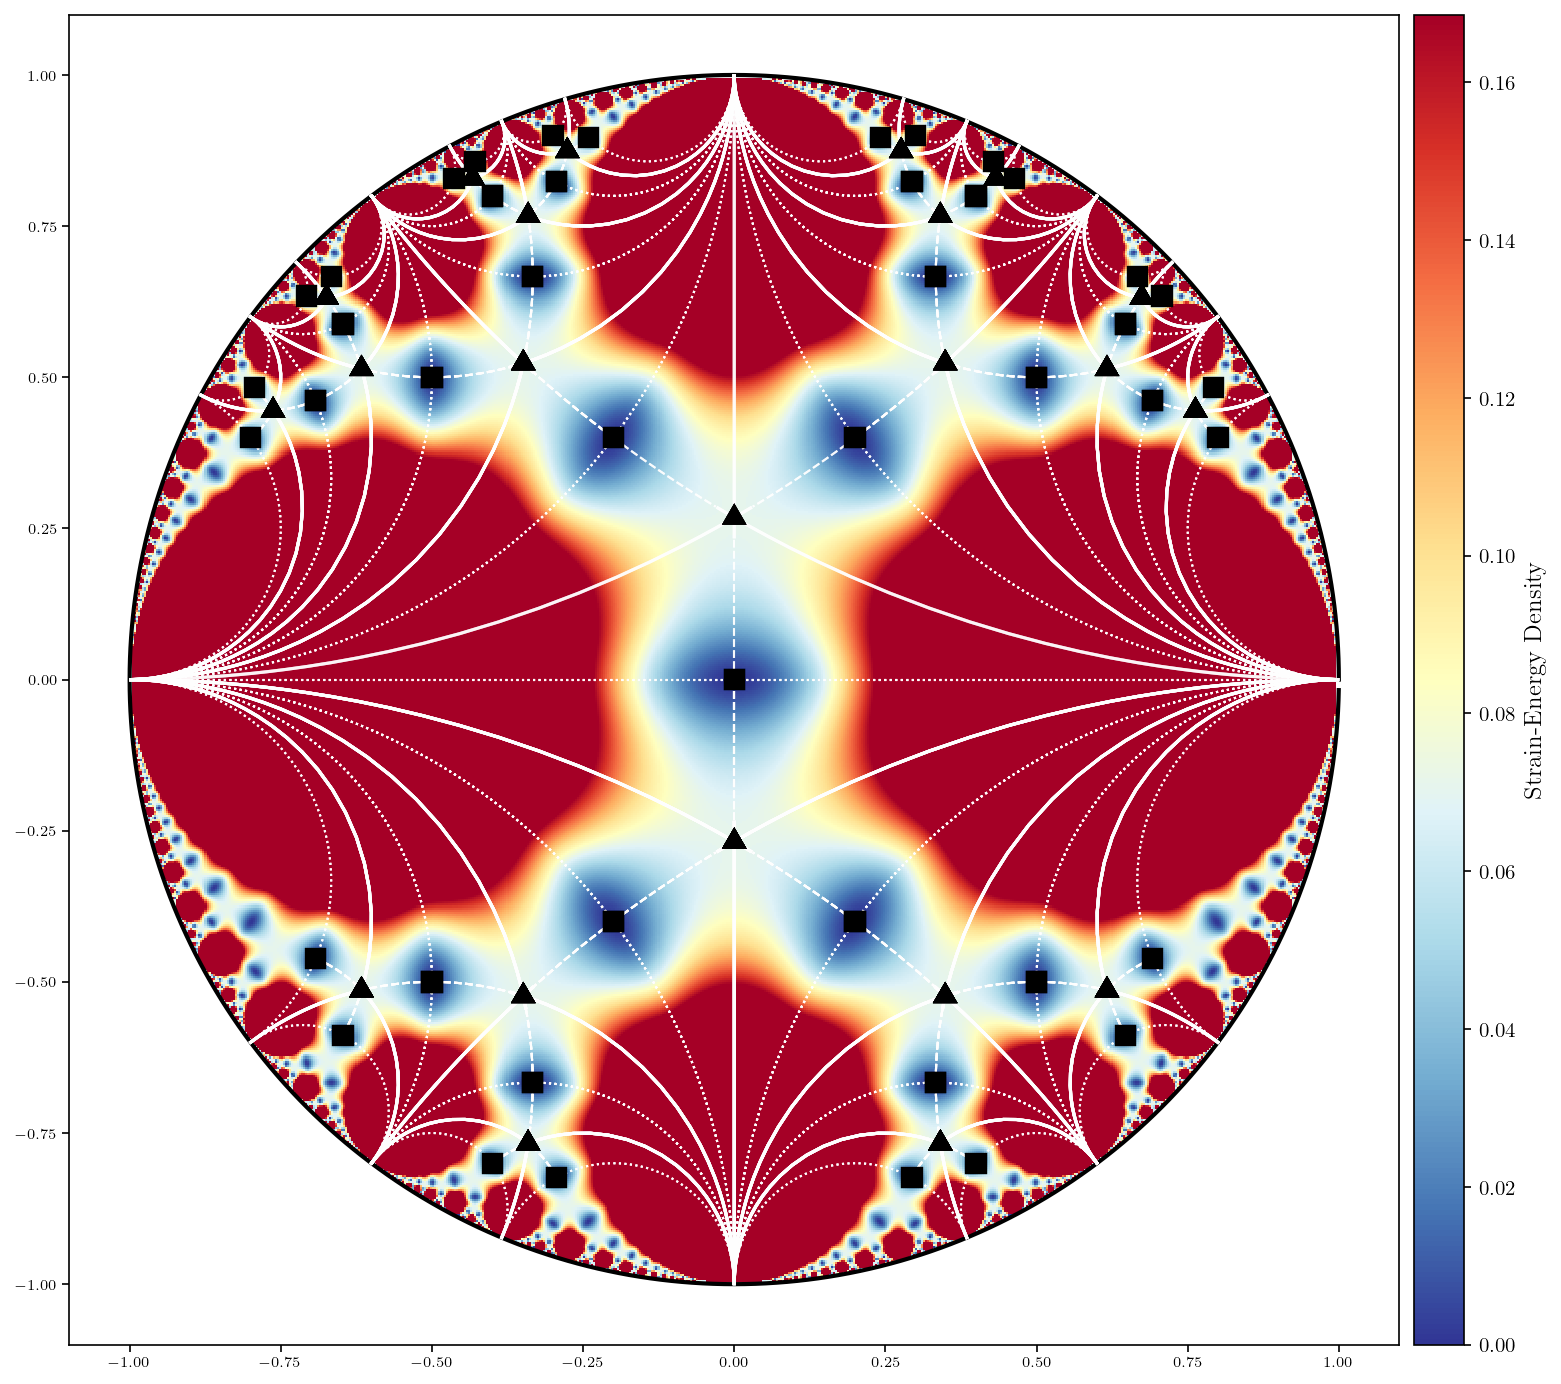
\includegraphics[scale=0.25]{figures_ordering/figure_02.png}}
\hspace{0.5cm}
\subfigure[]{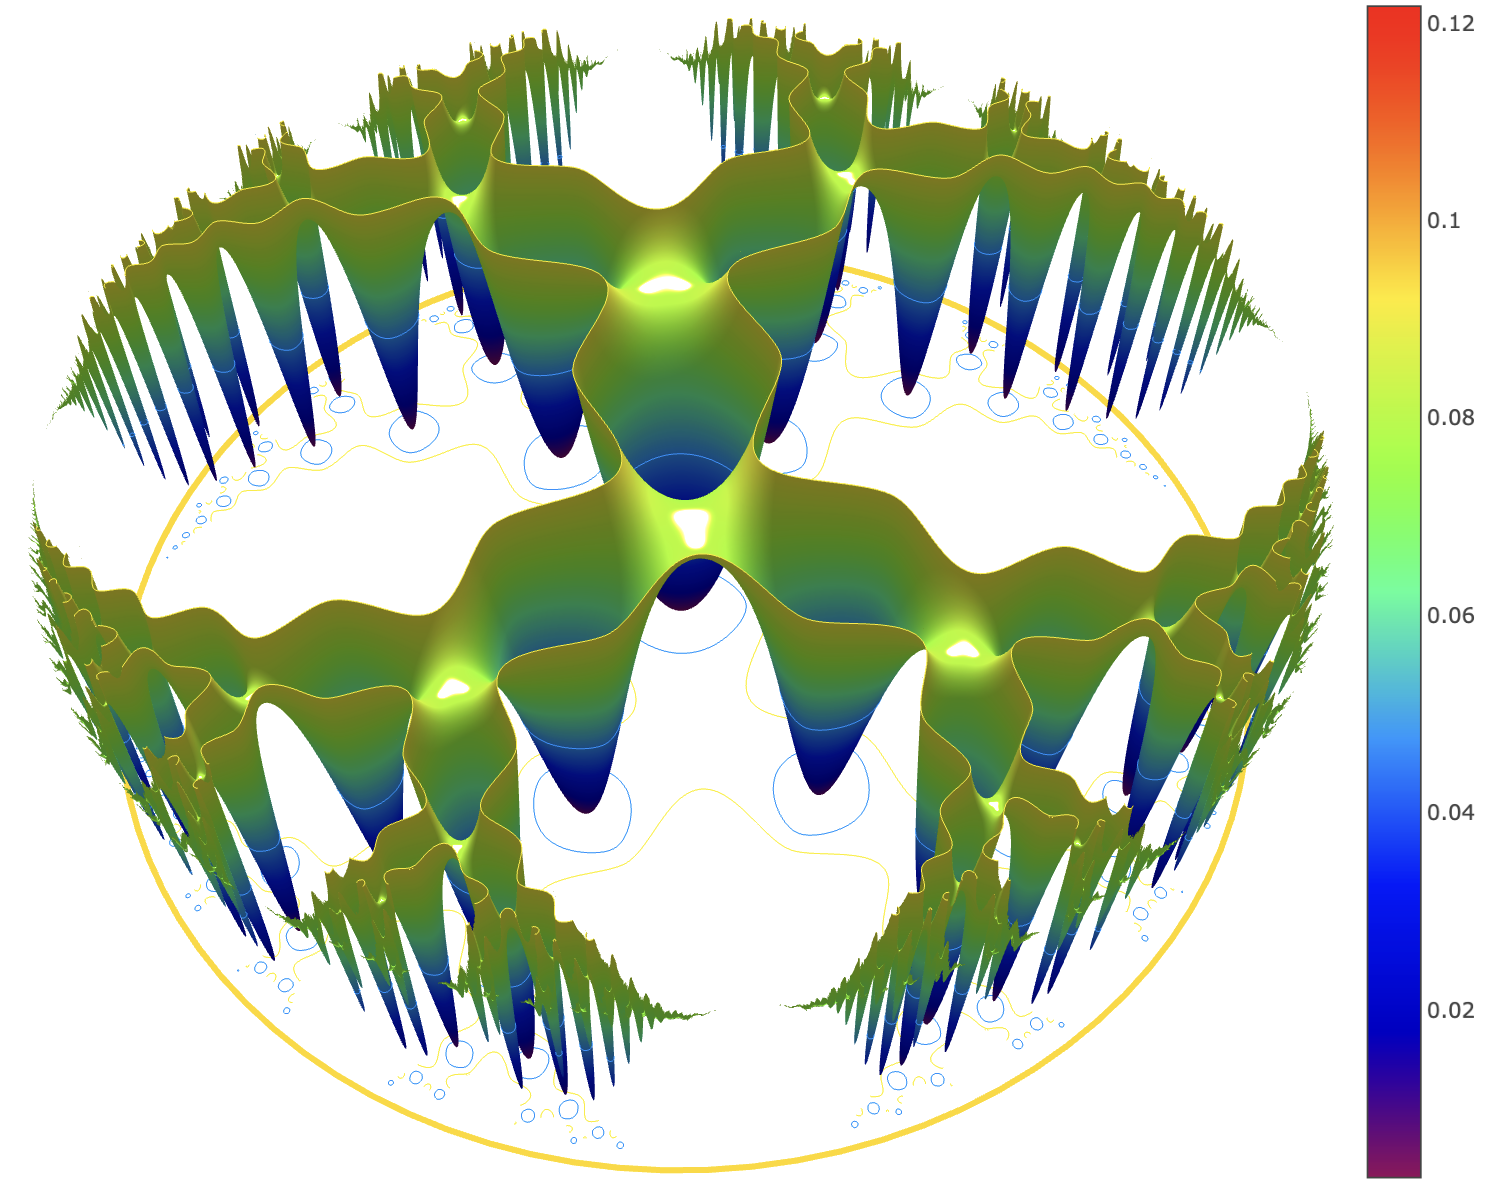
\includegraphics[scale=0.3]{figures_ordering/figure_03.png}}
\end{center}
\caption{Strain-energy density visualization in the configurational space of metric tensors using Poincaré disk coordinates. (a) Tessellated representation showing the discrete sampling of the strain-energy density field. (b) Corresponding continuous height plot of the strain-energy landscape over the same coordinate system.}
\label{fig:atlas1}
\end{figure} 
As we have already mentioned,   it is sufficient to define the energy density  only in one minimal periodicity  domain,  $D$ which is known in the mathematical literature on modular forms as a 'fundamental domain', see shaded domains in our Fig.~\ref{fig:atlas}(a,b,c). We shall refer to the restriction of the energy density to the fundamental domain   as $\phi_D(\tilde{\bf C})$ where $\tilde{\bf C}$ is the projection of  a  general ${\bf C}$ into this domain. We can write $\tilde{\bf C}={\bf m}^T{\bf C} {\bf m}$  where   ${\bf m}$ is the  corresponding  mapping  of the metric tensor ${\bf C}$ into  the fundamental   domain ensuring that  $ \phi({\bf C})= \phi_D(\tilde{\bf C})$.  

  In our 2D case, illustrated with better  resolution  in Fig. \ref{fig:atlas1}(a),  the fundamental domain   can be chosen  in the form ~\cite{Parry1998,Conti2004-sv,Engel2012,pitteri2002continuum}
\begin{equation}
\mathscr{D} = \left\{C \in \det{\bf C}=1, \quad 0<C_{11}\le C_{22},\quad 0\le C_{12}\le \frac{C_{11}}{2}\right\}.
\end{equation}
Given a generic metric $\bf C$, the task of finding a unimodular matrix ${\bf m} $ ensuring that $\tilde{\bf C}\in D$ (and therefore $ \phi({\bf C})= \phi_D(\tilde{\bf C})$) can be formulated in the form of a recursive algorithm known as Lagrange reduction~\cite{Conti2004-sv,Engel2012}. Specifically, if we define the matrices : 
\begin{equation}
{\bf m}_1=\begin{pmatrix}
1 & 0 \\
0 & -1 
\end{pmatrix},
\end{equation}
\begin{equation}
{\bf m}_2=\begin{pmatrix}
0 & 1 \\
1 & 0 
\end{pmatrix},
\end{equation}
and  \begin{equation}
{\bf m}_3=\begin{pmatrix}
1 & -1 \\
0 & 1 
\end{pmatrix}.
\end{equation} 
we can formulate the reduction process in a form of an explicit algorithm. Thus, if we start with an assumption that    ${\bf m} = \mathbb{I}$, we can  proceeds through the following steps: 
(i ) if $C_{12}<0$, change sign to $C_{12}$, ${\bf m}\rightarrow ${\bf m}${\bf m}_1$; 
(ii) if $C_{22}<C_{11}$, swap these two components, ${\bf m}\rightarrow ${\bf m}${\bf m}_2$;
(iii) if $2C_{12}>C_{11}$, set $C_{12}=C_{12}-C_{11}$, ${\bf m}\rightarrow ${\bf m}${\bf m}_3$. 
As a commentary, we note that the action of the matrix ${\bf m}_1$ is a reflection which returns an acute angle between two lattice vectors $\mathbf{e}_i$. The action of the matrix ${\bf m}_2$ is also a reflection as it swaps two lattice vectors $\mathbf{e}_i$. Both of these operations  belong to the point group and propagate the metric only inside the corresponding 'elastic  domain'  (Pitteri neighborhood)  composed of the four copies of the minimal  domain $D$ ~\cite{pitteri2002continuum}. Instead, the mapping defined by matrix ${\bf m}_3$ brings the metric outside the 'elastic domain'  and therefore represents a quantized analog of the macroscopic plastic strain ~\cite{perchikov2024}.




  
The single-period Landau potential $\phi_D(\tilde{\bf C})$ can be now constructed using the classical Cauchy-Born approach. Suppose   that material points in a representative volume $\Omega $ undergo an affine deformation  such that \begin{equation}
{\bf y}({\bf x}) = {\bf x} + {\bf u}({\bf x}),
\end{equation}
and the displacement vector  ${\bf u}({\bf x})$ is an affine function of $\bf x$, see Fig. \ref{fig:09}. Specifically, if we  define the vectors ${\bf R} = {\bf x} - {\bf x}' $ and ${\bf r} = {\bf y} - {\bf y}'$, connecting two atoms   in the reference  and in the deformed configurations, respectively,  we can write ${\bf r} = {\bf F} {\bf R}$ where we introduced the homogeneous  deformation gradient  $ F_{ia} = \partial y_i/\partial x_a = \delta_{ia} + \partial u_i/\partial x_a$. To compute the energy density $\phi(\bf C)$, we need to account for the elongation or shortening of   every  atomic bond and then average over the domain $\Omega $. Then, if the interatomic potential is $V(|{\bf r}|)$ which is defined within a given  cutoff,  
% = \sqrt{ R_1^2 C_{11} + 2 R_1 R_2 C_{12} + R_2^2 C_{22} })$, 
 we can write
\begin{equation}
\label{eqn:cg_sum}
\phi( {\bf C}) = \frac{1}{2\Omega }\sum_{{\bf x}} \sum_{{\bf x}'\in\mathcal{N}({\bf x})} V \Bigl( \sqrt{R_a C_{ab} R_b} \Bigr),
\end{equation}
where $C_{ab}=F_{ia}F_{ib}$ and the internal summations involves all points ${\bf x}'$ belonging to the cutoff neighborhood $\mathcal{N}({\bf x})$. After we compute the energy in this way inside the fundamental domain   $D$, we can extend it to the whole configurational space by $GL(2, \mathbb{Z})$ periodicity. The ensuing Landau potential can be expected to become smooth only in the limit when the size of the domain $\Omega $ tends to infinity.


\begin{figure}[h!]
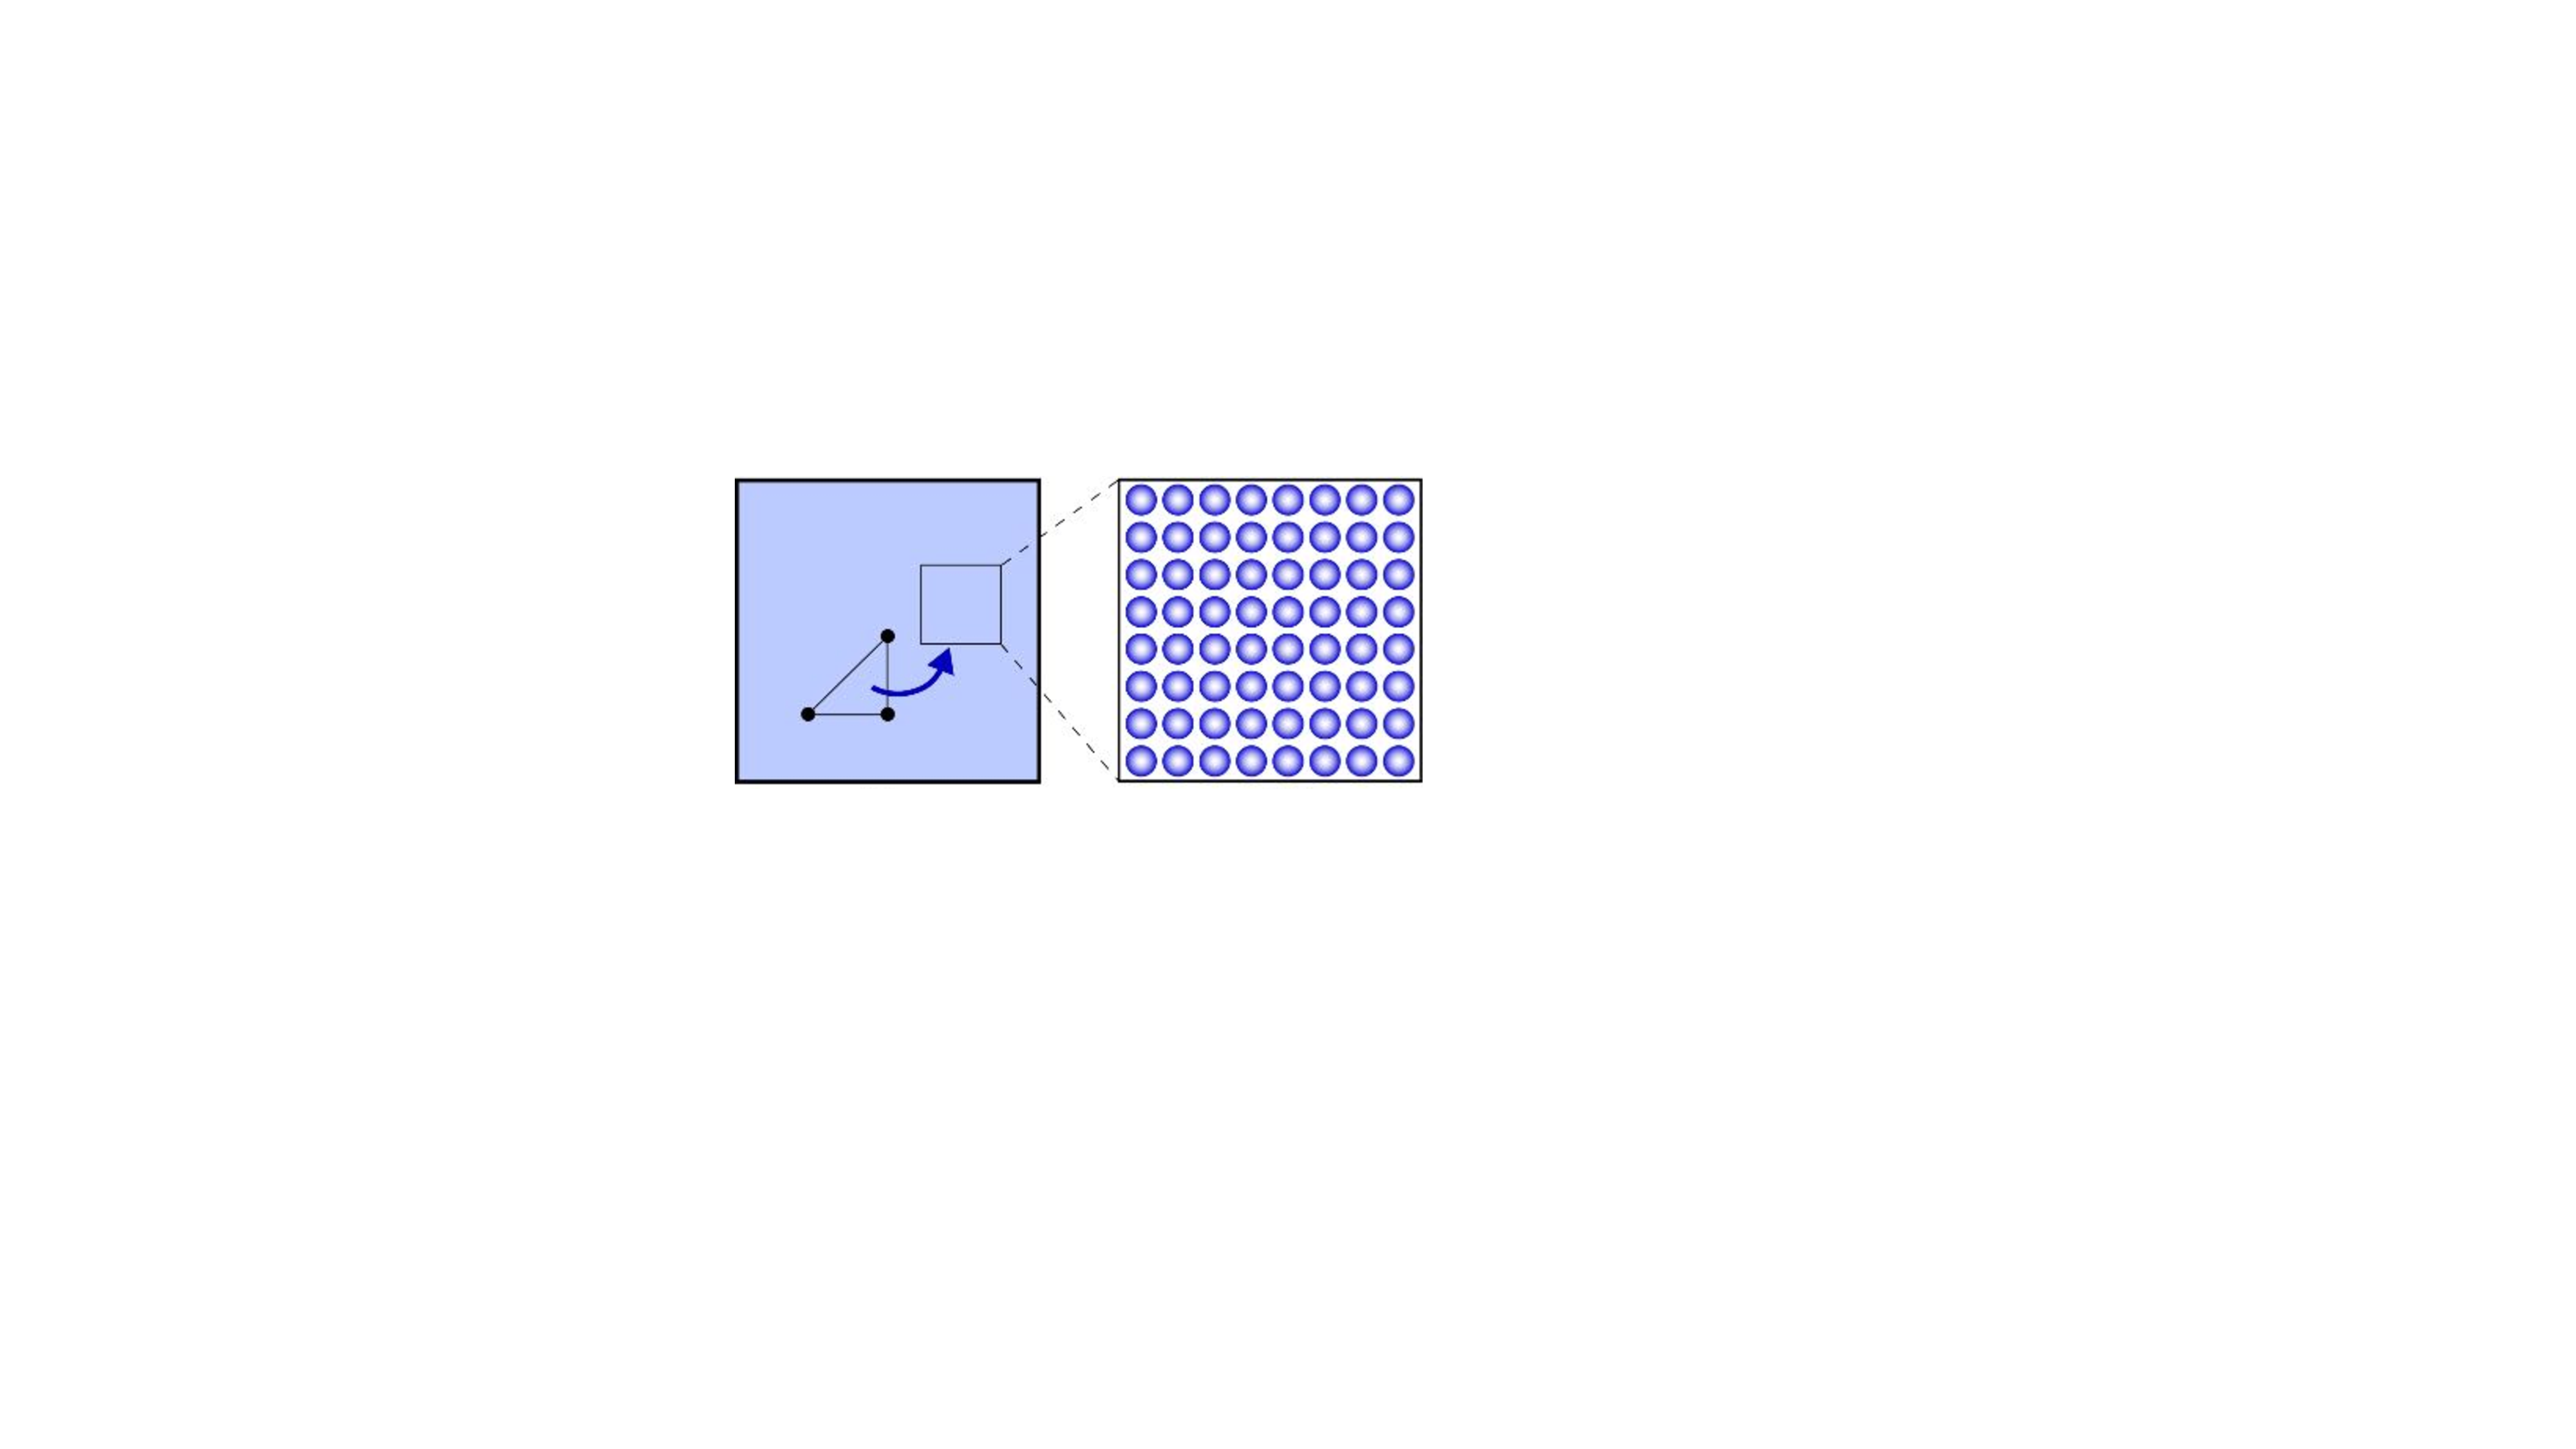
\includegraphics[width=0.275\textwidth]{figures_ordering/figure_04.pdf}
\caption{ Schematic representation of the finite element containing a number of atomic units which are assumed to deform homogeneously. ( \textbf{remove the triangle, show the inset as sheared, otherwise the energy is equal to zero})  } 
\label{fig:09}
\end{figure}

One can also achieve a desired level of smoothness phenomenologically, by representing  the energy density inside the domain  $D$ using  polynomial functions of different degrees.  In this work  we adopt , for simplicity, such an approach  and without relying  on any   particular interatomic potential,  use a prototypical   sixth order polynomial energy density developed in \cite{Parry1998,Conti2004-sv} which ensures stress continuity over the whole configurational space. 
Specifically, we assume that 
 \begin{equation}\label{enerC}
 \phi_0 \left( \frac{\tilde{\bf C}}{(\det {\tilde{\bf C}})^{1/2}} \right) = \beta\psi_1\left( \frac{\tilde{\bf C}}{(\det {\tilde{\bf C}})^{1/2}} \right) + \psi_2\left( \frac{\tilde{\bf C}}{(\det {\tilde{\bf C}})^{1/2}} \right), 
 \end{equation}
where 
\begin{align}
\psi_1 &= I_1^4 I_2 - \frac{41}{99} I_2^3 + \frac{7}{66} I_1 I_2 I_3 + \frac{1}{1056}I_3^2, \\
\psi_2 &= \frac{4}{11} I_2^3 + I_1^3 I_3 - \frac{8}{11} I_1 I_2 I_3 + \frac{17}{528} I_3^2.
\end{align}
and we introduced  the following hexagonal invariants of the metric tensor:
\begin{align}
I_1 &= \frac{1}{3}(\tilde{C}_{11} + \tilde{C}_{22} - \tilde{C}_{12}), \\
I_2 &= \frac{1}{4}(\tilde{C}_{11} - \tilde{C}_{22})^2 + \frac{1}{12}(\tilde{C}_{11} + \tilde{C}_{22} - 4\tilde{C}_{12})^2, \\
I_3 &= (\tilde{C}_{11} - \tilde{C}_{22})^2(\tilde{C}_{11} + \tilde{C}_{22} - 4\tilde{C}_{12}) - \frac{1}{9}(\tilde{C}_{11} + \tilde{C}_{22} - 4\tilde{C}_{12})^3.
\end{align}
The potential  \eqref{enerC} contains a single parameter $\beta$ that enables the enforcement of specific symmetries on the reference state. We select here  $\beta = -1/4$ which  ensures that global energy minimizers correspond to square lattices. The total elastic energy, allowing one to deal with both shear  and volumetric deformations, is taken in the form
 \begin{equation}
\phi(\tilde{\bf C}) = \phi_0 \left(\frac{\tilde{\bf C}}{(\det {\tilde{\bf C}})^{1/2}} \right) + \phi_v(\det \tilde{\bf C}). 
\end{equation}
 The volumetric part, which primarily influences dislocation core structures and controls the formation of voids, is assumed to be of a generic form
  \begin{equation}
 \phi_v(s) = \mu(s - \log(s)) 
 \end{equation}
 which prevents infinite compression. To maintain in our numerical experiments the strain field near the surface $\det C = 1$, we adopted   a sufficiently high value of the bulk modulus,  $\mu = 5$. 
  
In Fig. \ref{fig:atlas1}(b) we illustrate the resulting energy landscape  in the configurational space of metric tensors $\bf C$ with $\det{\bf C}=1$. It highlights the fact that any such  landscape would have  a network of low energy valleys along the directions representing simple shears along   crystallographic slip planes. It also reminds us that   the deepest energy wells  correspond  to the equivalent replicas of the reference square  lattice  furnished  by rank one deformation gradient tensors  representing lattice invariant simple shears. Instead, pure shear deformations  lead to extremely large elastic energy levels.

 

\subsection{Finite element representation}
\label{subsec:MTM_numerical_method}

The account for quantized lattice invariant shears makes the energy $\phi(\bf C)$ highly  non convex. Therefore,  the corresponding  continuum (scale free) problem is  highly degenerate.  In particular,  the energy minimization in such  continuum setting can be expected to produce infinitely fine microstructures \cite{Fonseca1987-pd}. In fact,  the lack of convexity of the potential is a property that the MTM   shares with other similar Landau type continuum theories. The usual way of regularization in this case  is  the introduction of  higher gradients (of the deformation, in our case) into the energy density and using the corresponding internal length scale as a cutoff parameter\cite{Hohenberg2015-jz}. This would be an approach of a phase field theory which often leads to over-regularization and the loss of sufficiently fine aspects of the microstructure which is acceptable near critical points but may compromise the inherent nonlocality by  treating it only in the long wave limit. Inside such a framework it is also a nontrivial task to represent  adequately the global lattice symmetry. In view of these limitations, in the MTM  approach we take a different path and bring  an internal  scale  into the model through  an explicit spatial discretization. Essentially, we  reduce  the space of admissible deformations to a finite dimensional set of compatible, piece-wise affine mappings.  

 More specifically, we   assume that   a crystal can be represented at the  mesoscale by a collection of $N \times N$   discrete elements organized in a  mesoscopic lattice  which preserves the symmetry of the atomic lattice. The   original lattice is effectively coarse-grained with an introduction of a uniform mesoscale grid.  The deformation is assumed to be piecewise linear and the   elastic  response is attributed   to   discrete material elements  whose linear size $h$ is viewed as a  physical parameter of the model. The numerical implementation of MTM is then based on solving an elastic finite element problem, with elements imitating mesoscopic aggregates  of atomic cells.  To trace the mechanical response of the crystal we follow the displacements of the   network of discrete nodes  labeled by integer valued coordinates $I =1,..., N^2$.

We assume further that each  of the  elements  is a deformable triangle and  employ standard finite element discretization with linear triangular 3-node elements  \cite{Irons1966} . We begin by  writing  the displacement field  inside each of these triangles  in the form 
\begin{equation}
 {\bf u} ({\bf z}) = \sum_{a } \mathcal{N} ^a({\bf z};h) {\bf u}^a,
 \end{equation}
 where ${\mathcal N}^a(\bf z;h)$ are   compactly supported  linear shape functions,  ${\bf u}^a$ are the amplitudes of the displacements of the nodes and summation is assumed over repeated indexes; the interpolation functions for each element are defined in terms of   local  dimensionless coordinate system. The mesoscopic deformation gradient is then 
 \begin{equation}
 {\bf F}({\bf z}; h) =\mathbb{I}+ {\bf u} ^a\otimes\nabla\mathcal{N} ^a({\bf z};h). 
 \end{equation}
 In terms of macroscopic reference coordinates,  the elastic energy inside each element can be  computed using the simplest   quadrature scheme 
\begin{equation}
w ({\bf x}; h)=\frac{1}{2}  \phi({\bf F} ({\bf x}; h)) J({\bf x},h),
\end{equation}
where $J$ is the determinant connecting local ($\bf z$)   and global ($\bf x$) coordinate systems (\textbf{ correct?}). 
 
We illustrate in Fig \ref{fig_08} our computational mesh which  is  a 2D   lattice representing a scaled version of the  original atomic lattice; a representative  triangular  finite element is, for instance,   the element BAC adjacent to the node A.  This element connects  three nodes and therefore the index $a$  associated with this element takes three values  $a=1,2,3$. We effectively assume in the MTM that the energy associated with  the deformed element BAC depends on the three parameters:  the deformed lengths  of the bonds AB and AC and   the deformed value of the angle BAC. To obtain these dependencies we use the Cauchy Born rule. Behind it is the assumption  that the element deforms as if it was embedded into   an infinite lattice undergoing a global affine (homogeneous) deformation. The latter is   fully characterized by the same three parameters which we interpret as the components of the corresponding metric tensor $C_{11}$, $C_{22}$ and  $C_{12}$.
\begin{figure}[h!]
\centering
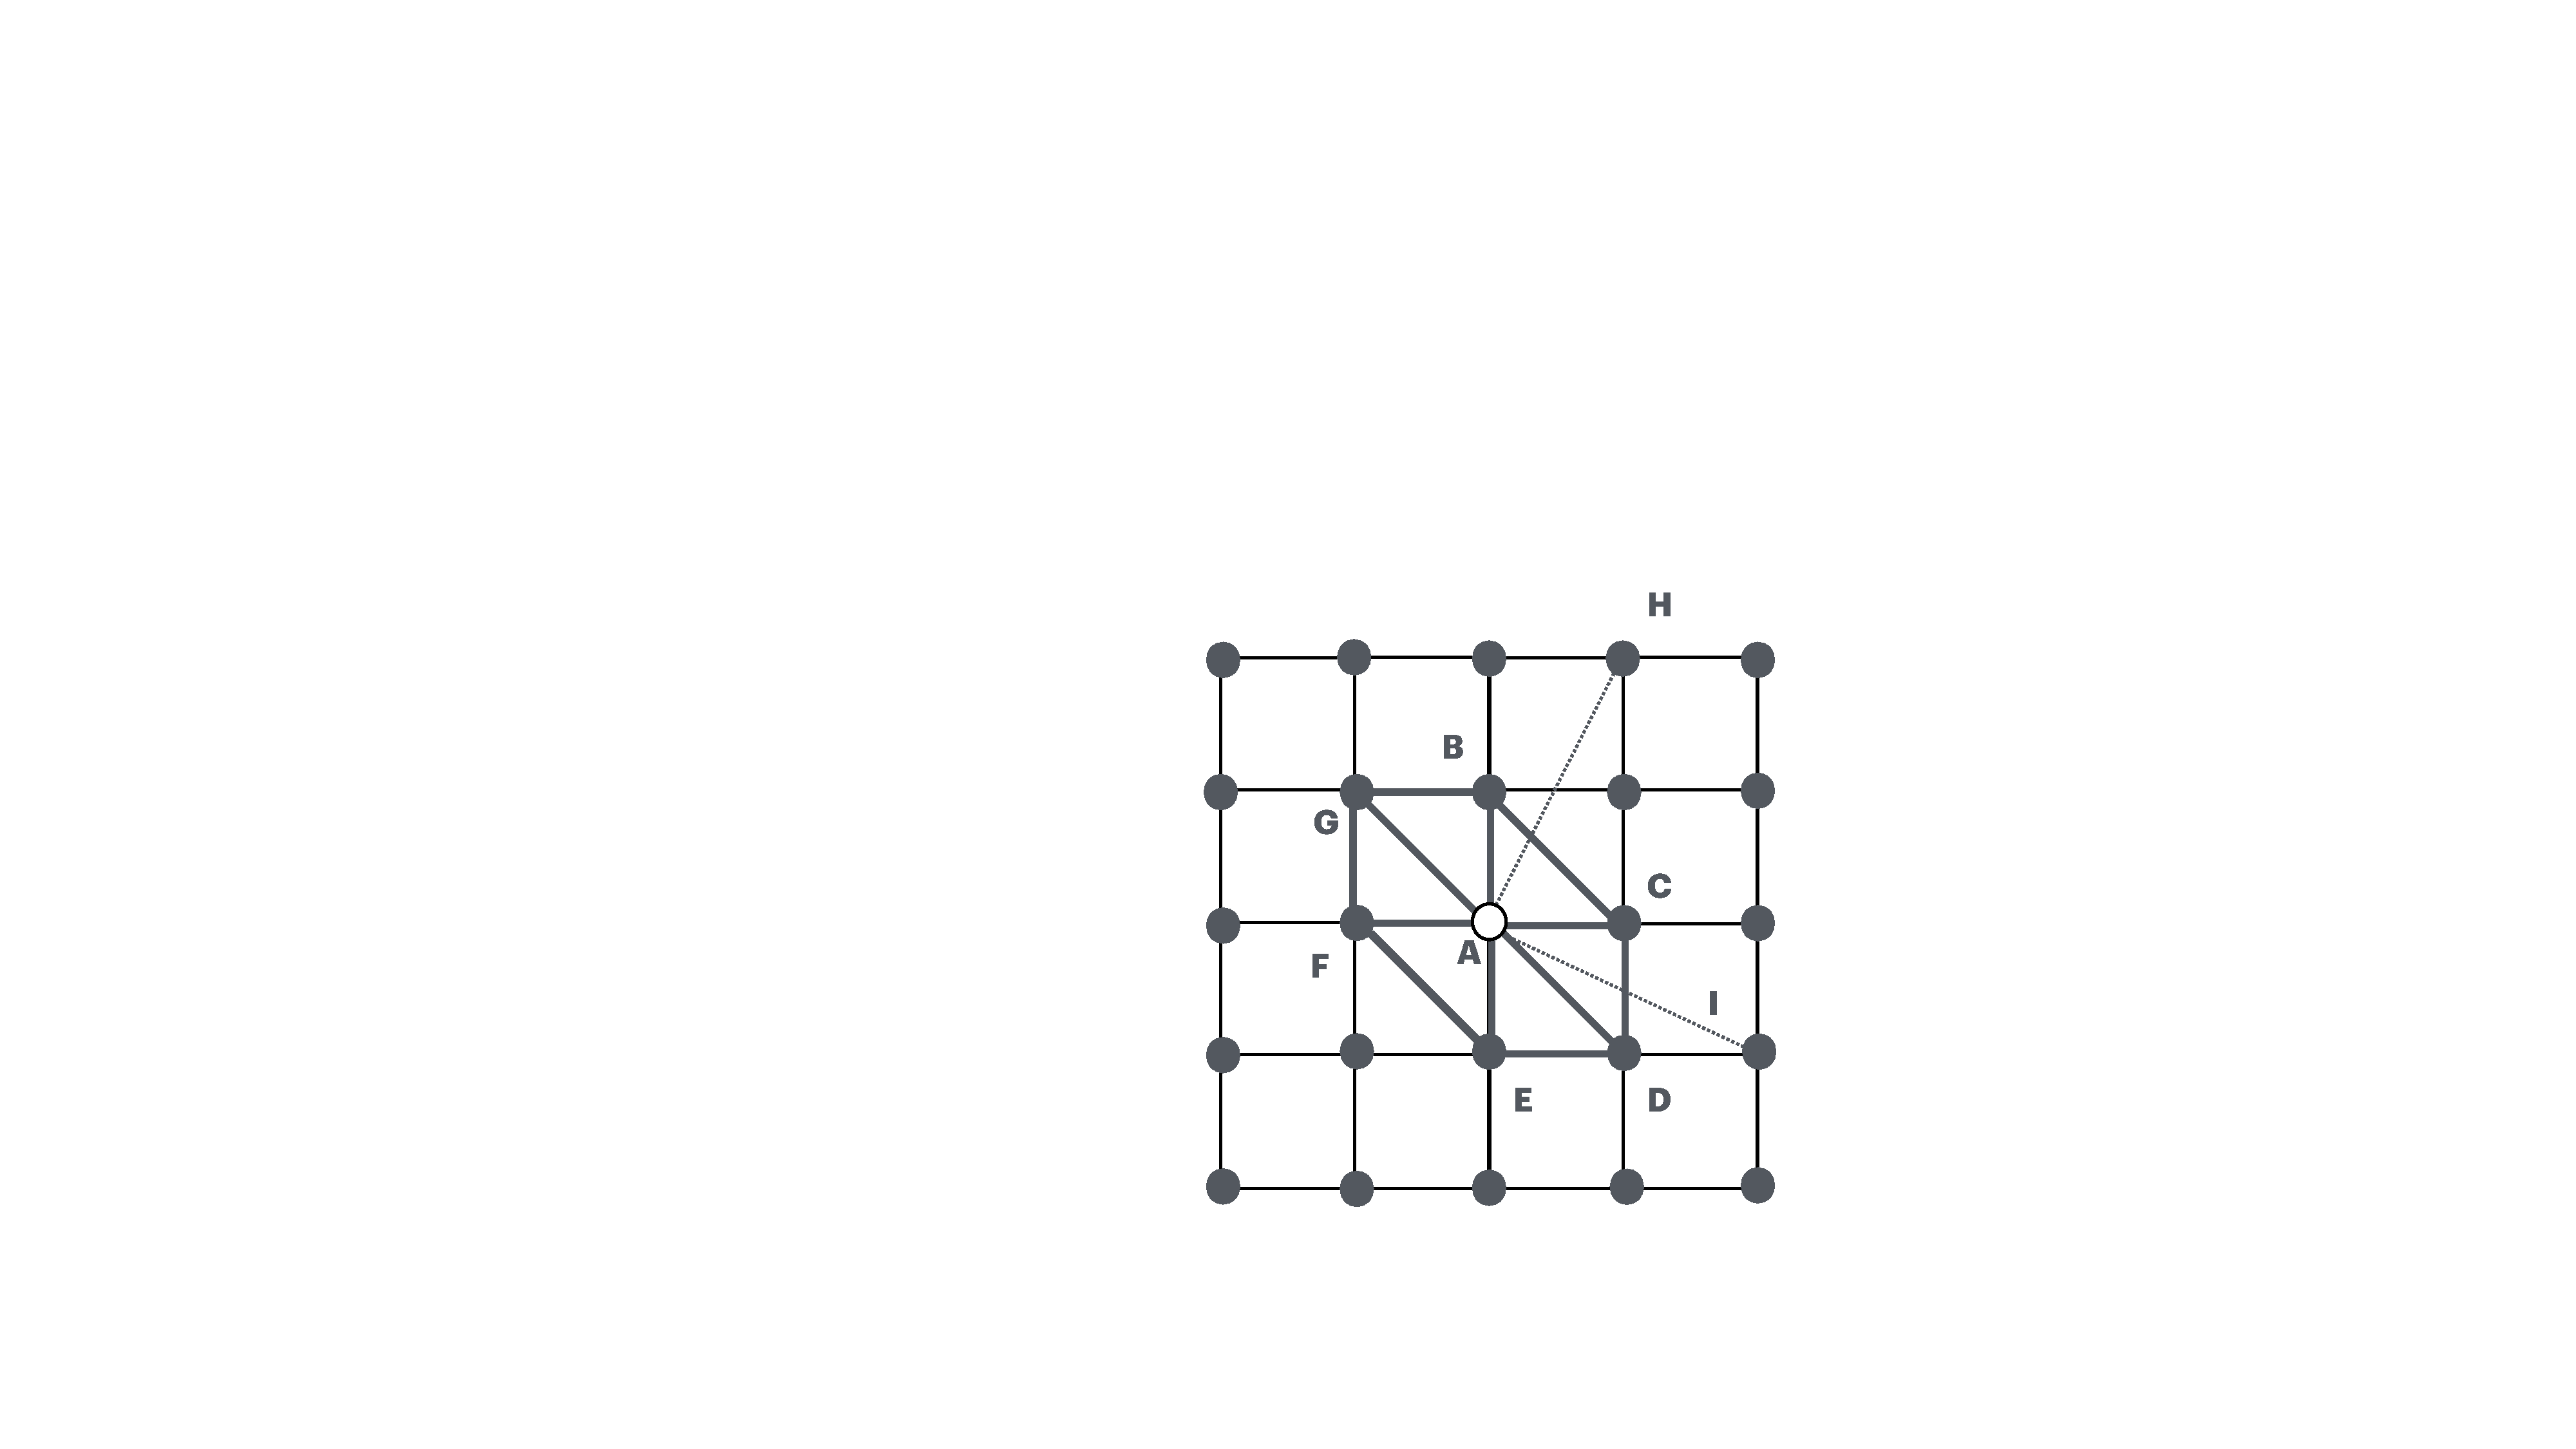
\includegraphics[width=0.2\columnwidth]{figures_ordering/figure_06.pdf}
\caption{Six triangular finite elements which are immediately adjacent to a generic   node $A$. }
\label{fig_08}
\end{figure}
Finding  solution of an elastic problem implies  local minimization of the energy 
\begin{equation}
W=\int_{\Omega}w({\bf x}; h)  d\mathbf{x}, 
\end{equation}
which is prescribed on a triangulated  domain \(\Omega\).   The conditions of mechanical equilibrium, formulated   in terms  of the first Piola-Kirchhoff stress tensor 
\begin{equation}
\mathbf{P}= 2\mathbf{F} \mathbf{m} \frac{\partial w }{\partial \tilde{\bf C}}\mathbf{m}^T,
\end{equation} 
take the form 
$$\nabla\cdot\mathbf{P}=0.$$
In the finite elelment representation these  equations can be rewritten in the form
\begin{equation}
\frac{\partial W}{\partial \mathbf{u}^{a}}=\int_{\Omega} \mathbf{P}(\mathbf{x};h) \nabla \mathcal{N}^{a} (\mathbf{x};h) d\mathbf{x} = 0.
\end{equation} 

Referring again to our Fig \ref{fig_08}, we observe that the elastic  energy $w$ dependence on the displacement of the node A has six contributions from the six adjacent triangular elements BAC, CAD, DAE, EAF, FAG and GAB. Therefore, in this setting,  the node A interacts  not only  with all the  nearest   nodes B,C,E,F but also with some next to nearest neighbor nodes D and G.   This interaction can be still interpreted as 'local', for instance, as it   shown in Fig \ref{fig_08},  the node A does not interact with  mode distant nodes H and I. 
 The implied  'multibody' interaction suggests  that the energy of the node A depends not only on the distances to the corresponding  nodes  B,C,D, E, F, G  but also on the three-point configurations represented by the angles BAC, CAD, AED, EAF and AFG. In other words, the   force balance  for the node A includes  not only responses to the  elongation of the bonds but also the associated  three-body contributions. 

We emphasize  that such non-pairwise  interaction is a result of coarse graining. In this sense the MTM  approach is not  in any  contradiction with the fact that in the corresponding atomic model  the interaction between the actual atoms is pairwise while maybe extending far beyond nearest neighbors. Essentially, in  the  MTM approach  the energy of a single  elastic element (triangle in our case)  is  computed as if the surrounding deformation field was affine which means that the local  inhomogeneity of the deformation is underplayed.   

Note also that the MTM, with parameter $h$   equal to atomic scale and with nodes identified with actual atoms,   can be seen as an atomistic scale model in which the actual inhomogeneity of local environment of a given atom  is neglected even if the deformation of the element itself is properly accounted for. Such effective coarse graining allows can be used as a way  to save computational time but at the expense of misrepresenting some microscopic aspects of the problem. Still, despite the inevitable shortcomings accompanying  this type of approximations, the  MTM approach remains advantageous as an accelerated computational scheme allowing one to bridge the gap between continuum and atomistic descriptions.  The implied  acceleration is due to the fact that   one does not need to keep track of  all neighboring atoms of a given element as the   energy of the element can be computed  in a straightforward  manner  based only on the information about  the local value of the deformation gradient.   The acceleration comes, of course, at a price: in the presence of an internal cutoff 
length scale some aspects of a genuinely atomistic description are necessarily lost. 



The ensuing mathematical  problem can be solved numerically using  a quasi-Newton method accompanied by the Newton–Raphson (NR) "refinement" when the initial guess is too far from the solution for Newton–Raphson method to converge  ~\cite{Tadmor1996-qi}. It has the advantage of being computationally efficient as well as being able to handle nonconvexity of the problem by only dealing with positive-definite Hessian matrices. The numerical method performs the minimization of the energy functional  iteratively. In very general terms, it begins with an initial guess of $\boldsymbol{u}(\boldsymbol{x})$ and a given approximation of the \textit{inverse} Hessian matrix $H_0$ as well as known optimal  number $m$ of BFGS corrections to be stored. An iteration first finds a minimization direction by performing a (one-dimensional) line search and finding the optimal step-size. Next, the solution is updated along with other quantities necessary to compute the inverse Hessian matrix of the next step.  The algorithm differs from BFGS in the way it handles the inverse Hessian matrix, which is approximated/updated by $m$ corrections at each iteration.

 More specifically, in our numerical experiments to find ${\bf u}^a$, we first use the L-BFGS algorithm~\cite{Bochkanov2013-lk} which builds a positive definite linear approximation allowing one to make a quasi-Newton step lowering the total energy.   The   iterations continue till  the increment  in the advance of the total energy   becomes sufficiently small. The obtained approximate solution is then   used as an initial guess  ${\bf w}^a$ to solve, using LU factorization~\cite{Sanderson2016-ht,itensor},  the  equations for the correction  $\text{d}{\bf w}^a$
 around   an initial guess for the displacement field $${\bf u}^a={\bf w}^a +  \text{d}{\bf w}^a.$$  The corresponding  system of linear equations can be written in the form
   \begin{equation}
 K^{ab}_{ij}dw_j^b+R_i^a =0,
 \end{equation}
  where 
\begin{equation}
K^{ab}_{ij}= A_{ipjq}({\bf F}) \frac{\partial {\mathcal N}^a}{\partial x_p}\frac{\partial {\mathcal N}^b}{\partial x_q},\,\,\, R^a_i= P_{ip}( {\bf F}) \frac{\partial {\mathcal N}^a}{\partial x_p}.
\end{equation}
Note that here  we used the Eulerian $i,j=1,2$ and the Lagrangian $K,L =1,2$ indexes and assumed summation on repeated indexes.  
We also defined  
 \begin{equation}
 A_{iajb}= \frac{\partial^2\phi_D{({\bf \tilde C} )}}{\partial F_{ia}\partial F_{jb}}.
\end{equation}
 the tensor of tangential elastic moduli. We note that  the knowledge of the Eulerian acoustic tensor  
 \begin{equation}\label{Q}
 {Q}_{ij}=F_{la} F_{mb} A_{iajb} n_l n_m,
 \end{equation}
  where $n$ are vectors of the unit circle allows one to  formulate the criterion of an elastic instability of the corresponding continuum body  in the form \cite{Ogden1997-rf,Grabovsky2014-fb}
  \begin{equation} \label{detQ}
  det (\boldsymbol{{Q}})=0.
  \end{equation}  

In our numerical experiments we   started with a pristine (defect free) square crystal sample represented by $N\times N$ finite elements with $N=400$. We then loaded this system quasi-statically along one of the the principal slip direction by  applying an affine displacement field representing hard device loading.  Specifically,  we prescribed   on the  boundary of our square sample $\partial \Omega$ the   displacement field 
\begin{equation}
 {\bf u}(\alpha,{\bf x})= (\bar{\bf F}(\alpha )-\mathbb{1}){\bf x} 
 \end{equation}
which was applied to all  boundary nodes. The special applied deformation gradient 
 \begin{equation} \label{F}
  \bar{\bf F}(\alpha)=\begin{bmatrix} 1  & \alpha \\ 0 & 1 \end{bmatrix}
  \end{equation}
was chosen to represent  simple shear along an  “easy” glide direction with shear amplitude $\alpha$  serving as the loading parameter.  By changing this parameter in increments of order $10^{-6}$,  we incrementally advanced   the  loading, while  waiting  for the system stabilization after each loading increment.  Specifically, after each incremental advance of the parameter   $\alpha$, the  displacement field was updated  by our  energy minimization algorithm   which used the solution from the previous step as the initial condition.  As we have seen, the energy minimization required a succession of iterations which is natural to interpret as a 'fast-time' overdamped dynamic process  taking place at a fixed value of the loading parameter. The latter is then interpreted as  evolving in a  'slow-time' scale. We effectively assumed full time scale separation allowing the 'fast-time' internal iterations to continue at the given value of the loading parameter  till  the value of  the energy increment reached below a sufficiently small threshold. After the termination of the energy relaxation stage, the loading parameter was  advanced again. 
 
 
 








\subsection{General comments}
\label{sec:length_scale}

%In what follows  we present the results of a direct comparisons between the outcomes of some benchmark numerical experiments conducted in MTM and in MS frameworks.  As a  basis of such comparison we point to the fact that both types of models are based on the same microscopic model  relying on   pair interactions between atoms and  operating with  exactly the same interatomic potential.

Before we turn to the results of our numerical experiments, some general comments about the MTM approach may be suitable as the physical implications of these experiements depend on the chosen modeling framework.  

 Recall first that in molecular dynamics approach (or rather molecular statics  (MS) in our quasi-static loading case)  there is also a characteristic internal scale: the  interatomic distance $a$ which is a microscale parameter.  In the mesoscopic approach of the MTM  the   coarse-graining scale  $h$, defining the  cutoff beyond which the deformation is considered homogeneous (affine), is necessaril larger than $a$ since  the goal is to   accelerate the computations. Their relative  magnitudes  should be, of course, discussed in terms of dimensionless quantities.  Thus, if the size of the macroscopic domain is  $L$, its  division  into finite elements introduces a dimensionless internal scale   $ h = L/N $ where we recall that $N^2$ is the number  of the nodes in the mesoscopic finite-element grid. The analogous microscale parameter is $\epsilon=a/L$ and  while we are ultimately implying the limit $\epsilon \to 0$, $\delta \to 0$, we must assume that $\delta\gg\epsilon$.  To locate in this perspective  the  classical continuum approach, we recall that  $h$ can be interpreted as an effective  size of a 'continuum particle'.  The, to obtain the continuum limit we first implicitly perform the limit $\epsilon \to 0$ and recover in this way local constitutive response  by using, for instance, the  Cauchy-Born rule. Then, to obtain a scale free theory we  perform the second limit $\delta \to 0$. Essentially we consider  a double   asymptotics 
$
   \epsilon \to 0,  \delta \to 0 ,
$
with $\delta\gg\epsilon$ which implies that $a<<h<<L$ and the only remaining length scale is $L$, see Fig. \ref{01}. Instead, in the MTM approach we effectively consider only a single limit $ \epsilon \to 0$ which  allows us still to use the Cauchy-Born rule. We then avoid the second limit and maintain a  small but finite value of the parameter $\delta$ which then necessarily satisfies  the  constraint $\delta\gg\epsilon$. In this situation we have  $a<<h \sim L$ and both $h$ and $L$ survive in the  limit $a/L \to 0$, see  Fig. \ref{01}. In this sense the MTM is essentially a continuum theory with an internal length scale, like, say, phase field model and other similar 'quasi-continuum' approaches.  
 \begin{figure}[h!]
\centering
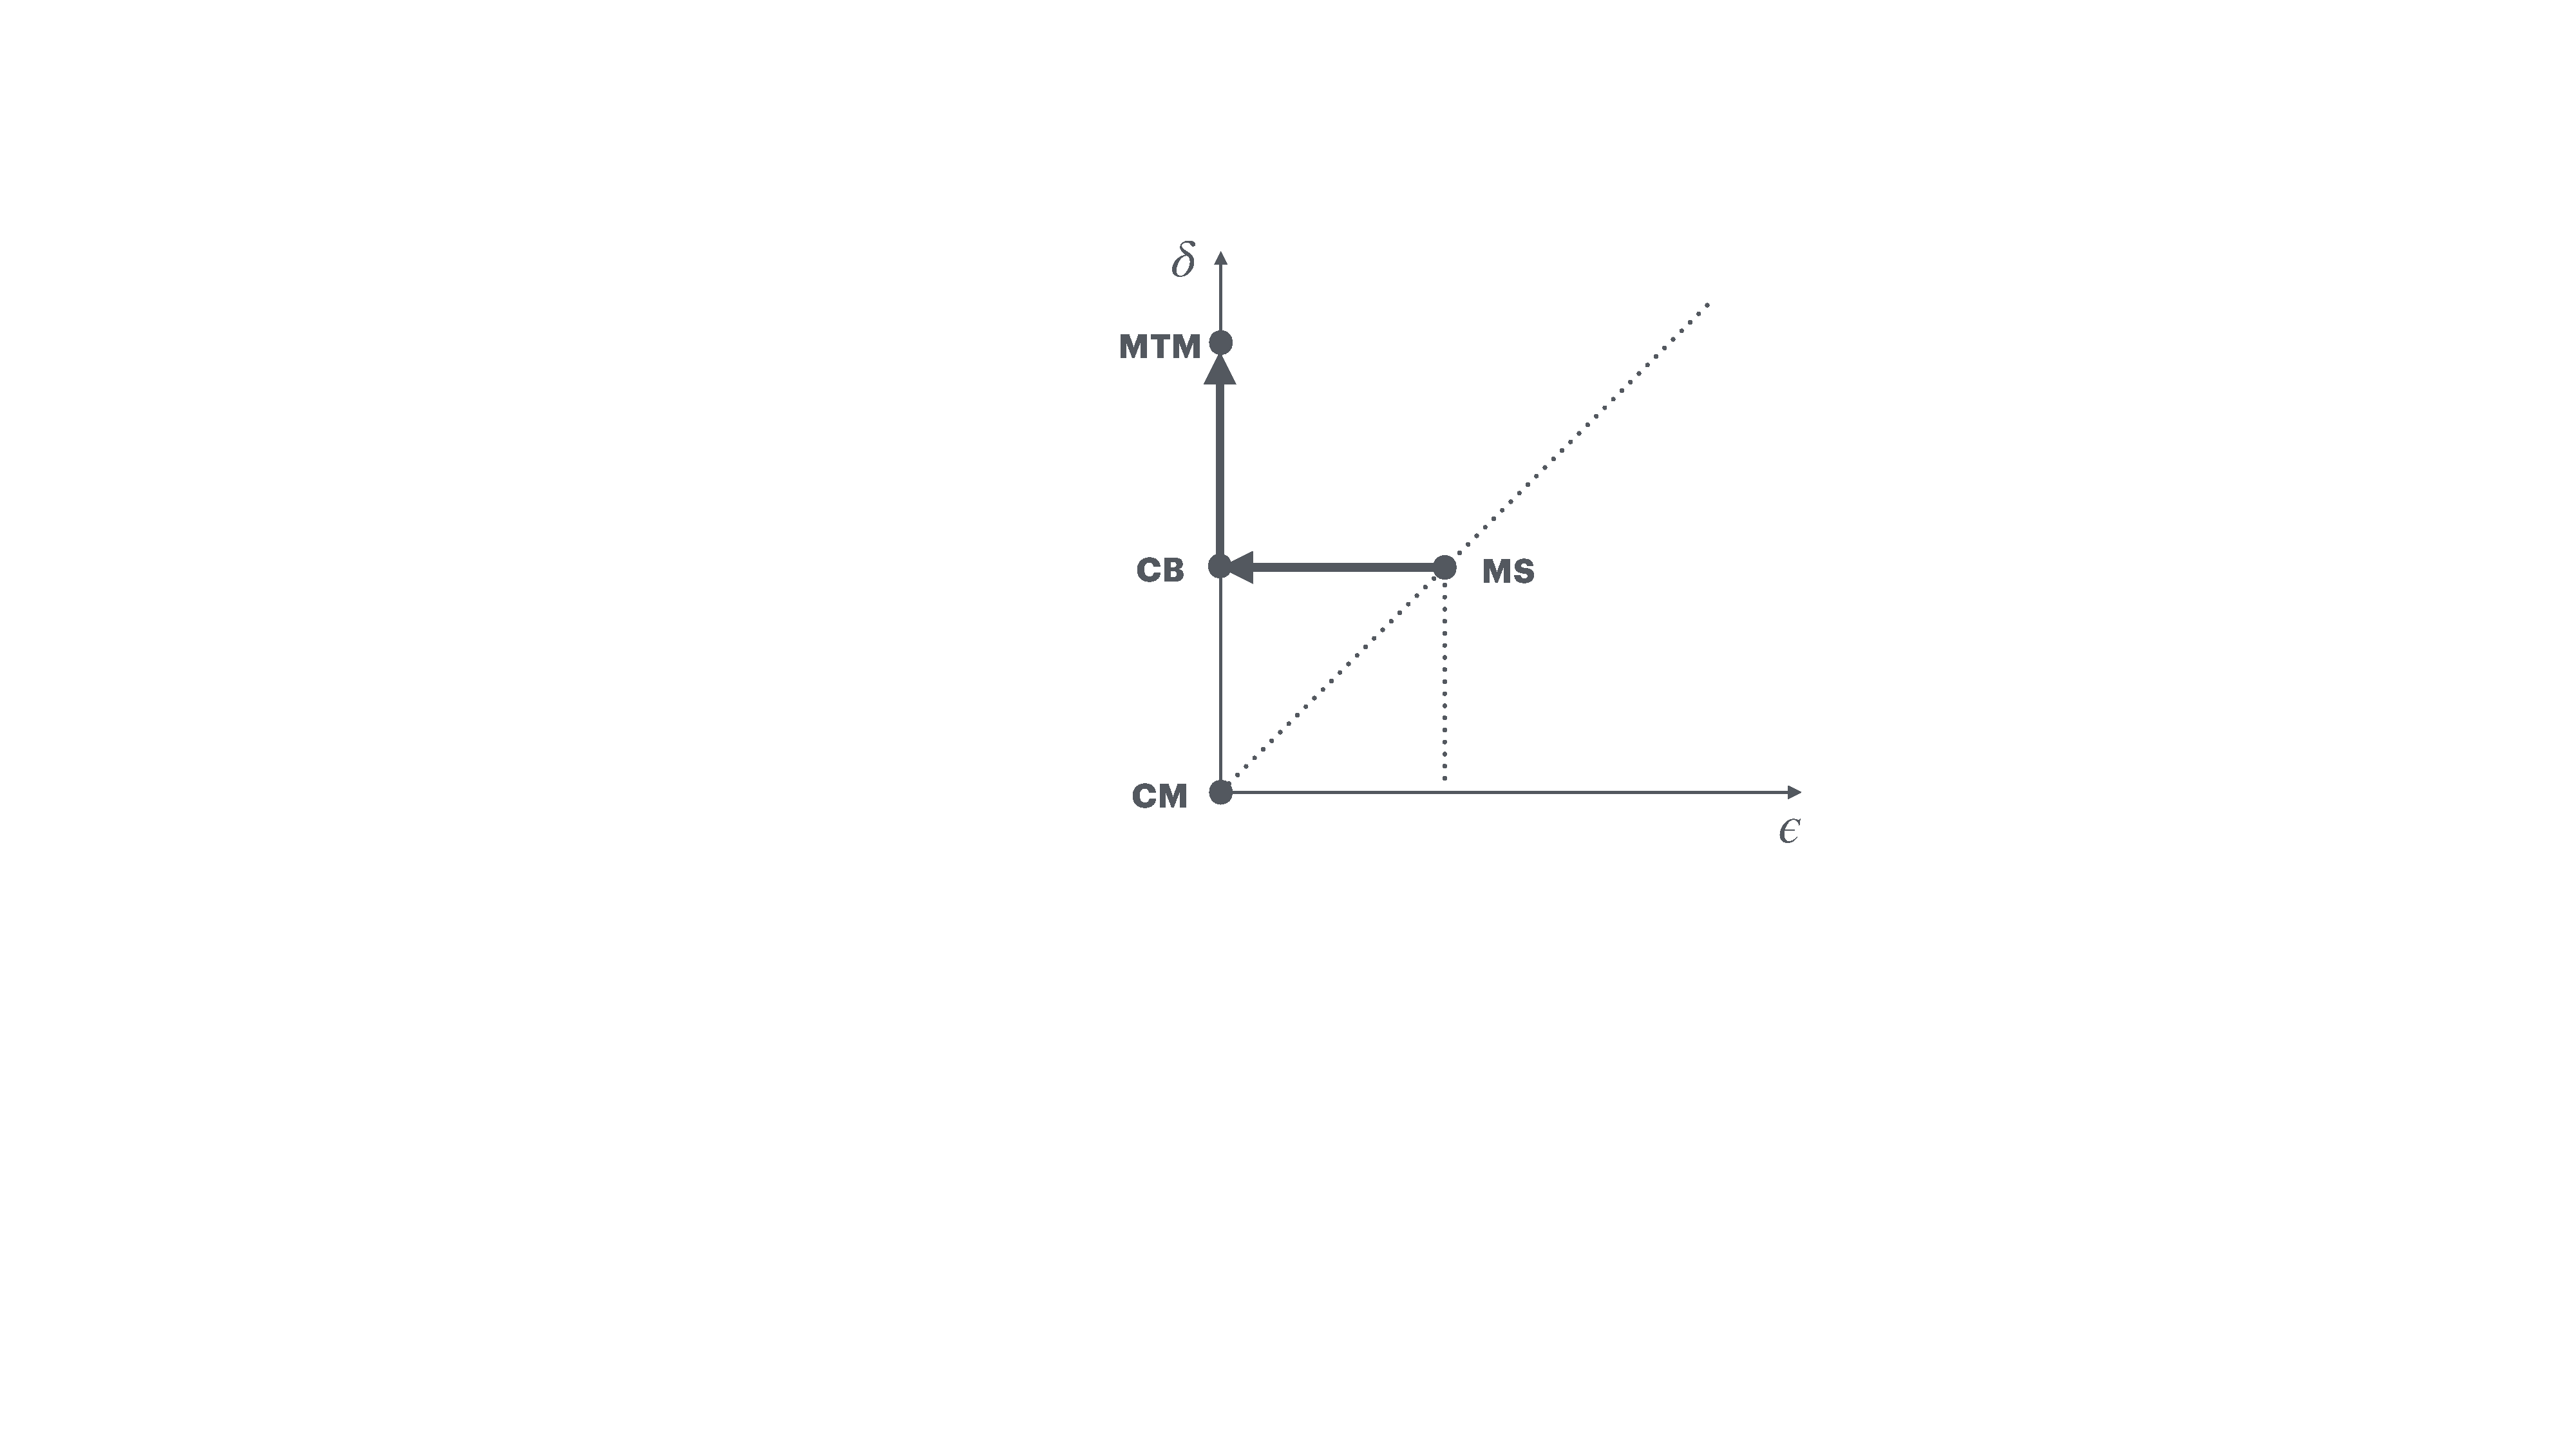
\includegraphics[width=0.25\columnwidth]{figures_ordering/figure_05.pdf}\caption{Schematic representation of the asymptotic ($\epsilon \to 0$, $\delta \to 0$) inter-relations between the molecular statics (MS), the continuum mechanics (CM) and the   mesoscopic tensorial model (MTM). As the (normalized) atomic scale $\epsilon$ tends to zero, the elasticity can be approximated by the energy density obtained through the application of the  Cauchy-Born rule (CB). If the mesoscopic scale  $\delta$ is eliminated, we obtain CM and if it is kept finite and  larger than the atomic scale, we obtain MTM.}
\label{01}
\end{figure}

As on all such theories,  making the dimensional parameter $h$ smaller is equivalent to making another dimensional parameter $L$ larger. In this sense the assumption  that $\delta$ is finite is equivalent to incorporating  finite size effects.  Thus,  even though changes in   $\delta $  will scale  the size of the core regions  of   dislocations, they  will  preserve the nature of  their long range  interactions, at least far away from the boundaries.  
 The use of Cauchy-Born coarse grained  description, will also  lead  to some  loss of   microscopic details in the description of dislocation cores,  however, the ensuing 'blurred' dislocations   will still   nucleate and self-lock adequately  even if  perhaps at different values of controlling parameters than in the corresponding MS simulations. Note also that at least some of the  characteristic   parameters including the core energy, the Peierls stress, the elasticity of a dislocation line, etc.,  may  be  matched by using $\delta$ dependent interatomic potential  which will then affect  the barrier structure in the corresponding  Cauchy-Born energy density.   The  situation here is the same as in the case of phase field description of phase boundaries where the need to reproduce  the realistic  value of the surface energy requires  the microscopic potential  to be appropriately re-scaled. 

 


 
  
  
Given the nature of the approximation provided by  the  MTM approach,  it can be compared  to other physical models with partial spatial resolution.  An important example is  the   model of turbulence known as  large eddy simulation (LES), e.g.   \cite{Sagaut2006,Davidson2009}. This  computational approach   deals with a similar problem  of choosing an ultraviolet cutoff  while  describing the processes at the smaller scales by  effective closure schemes.  The principal idea behind LES is the same as in the MTM approach: to reduce the computational cost by ignoring the smallest length scales which turn out to be the most computationally expensive to resolve. In both LES and MTM, the omitted small scale details   are  mostly sacrificed in the interests of addressing  the   scale invariant   aspects  of the phenomena. As in the MTM, the   sub-grid scales in the LES  are not  irrelevant, and their effect  is  modeled  by  sub-grid scale  models which  are not rigorously derived from the micro-scale but, instead, combine empirical information with some fundamental physical constraints. The choice of the grid size  in  LES  is rooted in  the idea   that LES accurately captures the energy-containing large eddies while modeling the smaller ones only effectively to maintain  a  balance between accuracy and computational feasibility. Similarly,  the choice of the cutoff  scale $h$ in the  MTM, where the sub-grid description reduces to Cauchy-Born type representation of the energy density,  is guided by the necessity to capture within  available  computational resources  the  collective effects involving a large number of dislocations leading to intermittent avalanche behavior  and  attendant spatial complexity. In this perspective,   the actual value of the parameter $h$ in the MTM approach is irrelevant as long as the \emph{quantitative} comparison with MS is not an issue and the computational domain is large enough so that the finite size effects due to interaction of   enlarged dislocation cores with   external boundary can be still neglected. In such settings, by changing $h$ we end up capturing  the same physical interactions even if they are viewed with different degree of resolution. 

 



Therefore, we adopt  a pragmatic  approach to the choice of the mesoscopic length scale $h$ and  make it problem-specific.  The idea is to  ensure  that  the  Cauchy-Born   energy density,  computed for a  \emph{finite} lattice fragment with  scale $h$,    can be considered as approximately periodic within  the interesting range of strains. In other words, we would like to  capture correctly  the  targeted  energy wells  while probably sacrificing the $GL(2,\mathbb Z)$ periodicity beyond the actually reachable range. Since the exact global  periodicity is recovered fully in the Cauchy-Born approach only in the limit of infinite sample size, our  strategy suggests that  the   cutoff scale $h$  should be increased  when  the goal is to capture the phenomenon of progressively larger slips along the same slip system. (\textbf{which value of $h$ are we actually choosing?})


 

 
Finally, it is important to stress that  despite its unusual, for plasticity theory, 'nonlinear elasticity' appearance, the MTM approach is  conceptually very close to the classical continuum plasticity (CP). For instance, both theories effectively account for the complexity of energy landscape by introducing low-energy valleys describing plastic `mechanisms'. However, if in CP, additional phenomenological  relations are needed to handle the coupling between different `mechanisms' \cite{Franciosi1985-cu,Cuitino2021-ps,Roters2010-rm,Dawson2000-ca,Bertin2023}
in the MTM approach, such coupling is automatic  as the model has  assess to the the height   of the energy barriers separating different low-energy valleys. It  also accounts for the barriers inside such valleys, moreover the   finite element representation, creates an even  broader set  of metastabile states.   A mechanical system driven elastically in the ensuing 'bumpy' energy  landscape   experiences a rich repertoire of snap-through instabilities which are ultimately behind the dissipative nature of the MTM.  Indeed, as we have already seen, such  instabilities are described implicitly by an overdamped model with relaxation time much shorter than the characteristic time of the loading. Therefore  the actual dissipative process is hidden inside the  local energy minimization protocol which hides   rate independent   plasticity behind the nonlinear elasticity appearance.




 \section{Numerical experiments}

\subsection{Periodic Boundary Conditions with Macroscopic Deformation}

\textcolor{blue}{To simulate an effectively infinite crystal under macroscopic deformation while maintaining computational tractability, we implement periodic boundary conditions (PBCs) through domain replication. The computational domain $\Omega_0$ with dimensions $L_x \times L_y$ is replicated in all spatial directions to create a periodic array of domains.}

\subsubsection{Translation Vectors and Domain Geometry}

\textcolor{blue}{We define a set of translation vectors $\mathbf{t}_n$ that generate the periodic lattice of domains:
$$\mathbf{t}_n = \begin{pmatrix} n_x L_x \\ n_y L_y \end{pmatrix}, \quad \mathbf{n} = (n_x, n_y) \in \{-1, 0, 1\}^2,$$
where $\mathbf{n}$ represents the integer lattice coordinates. For the 9-domain implementation, we consider all translation vectors within the immediate neighborhood of the central domain.}

\textcolor{blue}{Let $\mathbf{F}(t)$ denote the macroscopic deformation gradient tensor at time $t$. The position of any replicated domain relative to the central domain $\Omega_0$ is given by:
$$\mathbf{R}_n = \mathbf{F} \cdot \mathbf{t}_n,$$
where $\mathbf{R}_n$ represents the displacement vector of the origin of the domain corresponding to translation $\mathbf{t}_n$.}

\subsubsection{Particle Position Mapping}

\textcolor{blue}{For a particle located at position $\mathbf{x}_i$ in the central domain $\Omega_0$, its periodic image corresponding to translation vector $\mathbf{t}_n$ is positioned at:
$$\mathbf{x}_i^{(n)} = \mathbf{x}_i + \mathbf{R}_n = \mathbf{x}_i + \mathbf{F} \cdot \mathbf{t}_n.$$
This ensures that the macroscopic deformation gradient is consistently applied across all periodic images, maintaining the correct strain field representation.}

\subsubsection{Delaunay Triangulation and Triangle Selection}

\textcolor{blue}{After establishing the positions of all particles across the nine domains (original domain $\Omega_0$ and its eight periodic images), we perform a Delaunay triangulation on the complete set of particles:
$$\mathcal{P} = \{\mathbf{x}_i : i \in \mathcal{I}_0\} \cup \{\mathbf{x}_i^{(n)} : i \in \mathcal{I}_0, n \neq \mathbf{0}\},$$
where $\mathcal{I}_0$ denotes the set of particle indices in the original domain and $\mathbf{0} = (0,0)$ corresponds to the null translation vector. This means we deal with the all particles in the original central domain
and all periodic images of those particles in the 8 surrounding domains.}

\textcolor{blue}{From the resulting triangulation $\mathcal{T}$, we select only the unique triangles that have at least one vertex belonging to the original domain $\Omega_0$. The initial selection of all triangles with at least one node connected to the original domain may introduce duplicated triangles due to the periodic replication. Therefore, we apply an additional filtering step to remove these duplicates and retain only unique triangles.
This selection and filtering procedure ensures that:
\begin{enumerate}
\item Each triangle in the computational mesh is counted exactly once, eliminating redundancy from the periodic duplication
\item All triangles connected to the original domain are included, maintaining proper connectivity across periodic boundaries
\item The triangulation naturally incorporates the macroscopic deformation through the deformed positions of the periodic images
\end{enumerate}
}

\textcolor{blue}{The selected set of triangles $\mathcal{T}_{\text{unique}}$ forms the computational mesh for the mesoscopic tensorial model calculations, preserving both the periodic boundary conditions and the consistency with the applied macroscopic deformation gradient $\mathbf{F}$.}

In view of the pristine nature of our samples,  the initial phase of the deformation process,  starting at point $A$ in Fig. \ref{fig:02},   is necessarily  purely  elastic. During this stage, the  metric tensors  of all elements  remain  strictly  inside the elastic domain (Pitteri neighborhood). While the response of the crystal inside such a  domain could, in principle,  remain  homogeneous, the affine deformation becomes   unstable way before its boundary is reached.  The implied purely elastic instability   is preceded by the   elastic softening  and the actual instability  takes place near the maximal load. The  corresponding critical value of the loading parameter $$\alpha=\alpha_c$$   (\textbf{ provide  the actual value of $\alpha_c$})  can be well approximated  if we assume that the instability is associated with the loss of  positive definiteness of  the acoustic tensor \eqref{Q}. As we have already mentioned, the corresponding Legandre-Hadamard  conditions \cite{Simpson1989,Grabovsky2013,Steigmann2023}, indicating that the equilibrium equations of continuum elasticity stop being strongly  elliptic   at the corresponding affine configuration, are represented by \eqref{F}.  However, in view of the finite element nature  of our actual problem the solution of  \eqref{F}  provides only an approximation of  the critical value of the loading parameter with  the corresponding correction being of order  $(h/L)^2=N^{-2}$.  Note also that in  view of an pristine   nature of the crystal, at the critical value of the loading parameter (point $B$ in Fig. \ref{fig:02}) all finite elements can be expected to  become unstable  simultaneously. This would lead  to a nonphysical highly unstable behavior    and therefore, to observe a generic response we had to regularize the problem by  adding  at the   onset of instability  a small amount of quenched  disorder which  was removed right after the instability  took place.


  
\begin{figure}[ht!]
\centering
\includegraphics[scale=.2]{figures_ordering/figure_07.pdf}
\caption{ ( \textbf{change the order of a and b.}) Priming of the pristine sample  and first stage yielding.  (a) Strain-energy density evolution during proportional loading. The  labeled configurations are A (initial), B (first yielding point), and C (post yield). The sharp drop of energy from B to C represents the transition from pure crystal to an 'amorphous crystal', see the text for more details. The subsequent microplasticity regime takes place at almost constant energy. Colors in the inset indicate the level of energy density. (\textbf{correct?}). (b) Stress field $\tau$ (\textbf{what kind of stress it is?}) evolution along the same loading path. The instability takes place when the crystal reaches its  theoretical  strength threshold. The stress drops almost to zero opening the way to a hardening regime of 'microplasticity'.    The inset   illustrates the evolution of the corresponding dislocation density $\rho$. Here $N=400$ (\textbf{ correct?}) }  
\label{fig:02}
\end{figure}

  The overall macroscopic mechanical response before and during the instability is illustrated in Fig. \ref{fig:02}(a,b). As we have already said, the loading process begins in point $A$ where at zero applied stress (\textbf{ explain which stress component is plotted  here?}) the pristine crystal is undeformed and has zero elastic energy. The configuration continues to be homogeneous as the loading increases and we observe the nonlinear softening elastic behavior dictated by the chosen nonlinear elastic potential. Near the load maximum of the stress-strain curve (point $B$) we introduce a small quenched disorder. The resulting pre-instability  highly stressed  configuration  is shown in Fig.  \ref{fig:22}(a) where we show the energy distribution inside  individual  finite elements.  Note that this state is almost homogeneous, in particular, the imposed small stress modulation does not result in the formation of dislocations. 
  
   
Our next Fig.  \ref{fig:22}(b)  shows the post-instability configuration  (point $C$). One can see that   the breakdown of an   almost  affine elastic state  takes the form of a major  system-size  rearrangement transforming a perfect crystal into a dislocation-rich, apparently 'amorphous crystal'. Note that in the course of this  catastrophic  system-spanning event  the crystal   abruptly loses almost all its  accumulated elastic energy with stress   dropping almost to zero, see Fig.\ref{fig:02} (a,b).   The inset in  Fig.\ref{fig:02}(a) shows the jump of the dislocation density $\rho$ from zero in both configurations $A$ and $B$ to a finite value in the state $C$.  
\begin{figure}[ht!]
\centering
\includegraphics[scale=.35]{figures_ordering/figure_08.pdf}
\caption{Emergence of a quasi-glassy state.  (a) Highly stressed perfect crystal close to the first yield point (B) with small  initial quenched disorder introduced to break the unphysical degeneracy of the pre-yielding state.  (b) Post- (first)yielding   configuration (C) after   massive nucleation of  dislocations which self-organize into an intricate multi-scale   pattern. Colors indicate the level of energy density. ( \textbf{correct?})}. 
\label{fig:22}
\end{figure}
  
  The  deformation pattern  emerging after the stress drop (point $C$),  reveals   \emph{collective}   nucleation  of a huge (\textbf{how many?})  number of dislocations. The latter were identified  using the classical Delaunay triangulation method. It  allowed us  to detect  the coordination number anomalies and 5/7 coordination defect pairs were interpreted    as dislocations. One can say that  an artificially created    defect-free  (cold) sample was converted  into a  generic (hot)  sample carrying  a realistic initial distribution of defects, see Fig. \ref{fig:22}(b).  We call such 'preparation' or 'priming' realistic because  the  defects  are not placed by hand but instead emerge in the course of self organization. The corresponding  highly cooperative  event unfolded dynamically  in a fast computational time involved in local energy minimization.   In other words, one can say that  the achieved configuration is  the first stabilized state   reached by an overdamped relaxational dynamics involving   nucleation and annihilation of dislocations as well as the formation of dislocational entanglements. It is then natural to expect that the attained  state is only marginally stable which is an observation which we discuss in more detail in what follows. 
  
Note next that while the observed catastrophic  mechanical response  is still associated with \emph{plastic} deformation, its  discontinuous nature  is highly reminiscent of brittle fracture. The phenomenon of  plastic brittleness in crystal plasticity is  realistic,  moreover   it has been qualified as  a characteristic feature of sub-micron crystal samples with high initial purity (absence of solutes, precipitates, and dislocations).\cite{bei2008effects,chrobak2011deconfinement,wang2012pristine,Cui2017-xn,Greer2011-hi,Brenner1956-rx,Brenner1958-dr,Sharma2018-iw,Mordehai2018-qm,Lilleodden2006-jq,Corcoran1997-vt}. However, as we discussed in the Introduction, such discontinuous yield  is also reminiscent of the  mechanical response  of well-annealed glasses.  In particular, we have seen that among other amorphous systems which exhibit similar quasi-brittle behavior  are there are  jammed configurations of  granular media which  are only marginally stable. In this perspective, the dynamic  process, transforming the  pre-avalanche configuration $B$ into the  post-avalanche  configuration $C$,  can be viewed as  converting an unstable  'fluidized' system into a marginally stable one. In view of its highly disordered appearance, which of course does not indicate the absence of correlations,  and in the absence of other established choices,  we refer to this state as the 'amorphous crystal'. 
\begin{figure}[h!]
\includegraphics[scale=.2]{figures_ordering/figure_09.pdf}
\caption{Post- (first) yielding deformation history: a typical stress vs. strain curve and and the corresponding  dislocation density in a system with $N=400$ (\textbf{ correct?}).  The hardening stage from $D$ to $F$ shows the pre-(second) yield 'microplastic' deformation. The transition from $F$ to $H$ correspond to a cluster of system spanning avalanches. The post-(second) yield stationary plasticity regime is represented by the state $I$ on a stress plateau.}
\label{fig:2}
\end{figure}

 

After such   \emph{preparation}  stage, we continue to apply the same  athermal quasi-static loading  protocol to the emerging  'glassy' system.  Specifically,  we subject our  highly dislocated crystal to progressively larger simple shears.  The ensuing stress-strain response  is illustrated in Fig. \ref{fig:2}. Its salient feature   is  the presence of   irregularly placed elastic branches   interrupted by abrupt  stress drops. The latter represent intermittent  plastic avalanches  which  involve partial or complete unlocking of  dislocational structures;  the associated dynamic  restructuring of the deformation pattern may be  either local or global.


In  Fig. \ref{fig:2} we can identify  two rather different regimes.
 The first regime shows plastic hardening behavior and is represented by the configurations $D$, $E$ and $F$. In this regime the dislocation density remains almost constant.
% by first slightly decreasing (from $D$ to $E$) but then showing equally slight growth (from $E$ to $F$).  
 Then there is a localized major multi-stage stress drop represented by the transition $F \to G \to H$.  During the associated system spanning restructuring event   the dislocation density abruptly jumps.   Finally there is a  quasi-stationary  regime of an 'easy glide type' represented by a stress plateau and exemplified by the state  $I$.
According Fig. \ref{fig:2}, in the  'hardening' regime  the dislocation density remains almost constant. In this regime the dislocation density  progressively increases. 
 
\begin{figure}[h!]
\includegraphics[scale=.3]{figures_ordering/figure_10.pdf}
\caption{Post-(first)yielding which is also a pre-(second) yield deformation history: hardening regime representing 'microplasticity'  with almost constant dislocation density and with major dislocation self-locks (entaglements) between the states $D$ and $E$ remaining intact. Colors indicate the level of energy density. ( \textbf{correct?})}
\label{fig:03}
\end{figure}

 The observed   yielding behavior is  highly reminiscent of the plastic  response of well annealed ' brittle' glasses. To understand it better we now turn to the analysis of the corresponding  spatial dislocational micro-configurations.
 
 
In Fig. \ref{fig:03}  we show the  energy distributions in the states  $D$  and $E$;  note that the highest energy levels  correspond to the location of dislocation cores. One can see that during the transition $D \to E$  no  grain boundaries or shear bands,  appear to be forming. Only  preexisting mobile dislocations  are  moving between the  locking sites formed by immobilized dislocations.   One can say that  dislocations, which remain mobile after the first massive dislocation nucleation event, are confined inside the effective cages where they can pile up but from where they can only rarely escape by  breaking the  existing locks. 
 
 
Note next that in this regime  both major slip systems are activated and  small dislocation avalanches,  corresponding to to weakly coordinated dislocation motions along their gliding planes, are abundant.  The characteristic  entanglements involve  dislocations on two diffefrent slip planes transiently blocking each other.  The processes of nucleation and annihilation of dislocations  motion appear to be  largely suppressed.  in Fig. \ref{fig:22} we see that  even though beyond the state $C$ the system exhibits stress-hardening behavior,  the energy remains  almost unchanged. This means that the work of the loading device is almost all converted into heat  as the dislocation number remains basically fixed. 

%and  not of a collective nature in contradistinction to what we have seen during the first  catastrophic system-size avalanche. In fact, already

Overall, such pseudo-elastic regime preceding macroscopic yield  can be interpreted as micro-plasticity. It is represented by local plastic events that individually do not lead to statistically meaningful changes in dislocation structure and are usually not 
 resolved in conventional bulk deformation experiments.  However,  this  small-scale  intermittent  micro-plastic  activity  which usually becomes apparent  only  in samples of  reduced size, is still  characteristic of pre-yield behavior for  both crystal and glassy systems  \cite{Maas2018-qu,Papanikolaou2017-ld,Sparks2018-zp,sparks2019avalanche,Rizzardi2022-iz,Duan2023-ue}.

\begin{figure}[h!]
\includegraphics[scale=.25]{figures_ordering/figure_11.pdf}
\includegraphics[scale=.278]{figures_ordering/figure_12.pdf}
\caption{Second stage yielding represented by the system size restructuring of a dislocation pattern. Major shear band forms between the states $G$ and $H$. Colors indicate the level of energy density. ( \textbf{correct?}) }
\label{fig:031}
\end{figure}

 
We now  turn to the macroscopic yield which we associate with the second major  restructuring event starting at point $F$. The whole  system-size avalanche  takes the form  of a two-stage  transition  $F \to G \to H$. The corresponding snapshots of the  spatial dislocational micro-configurations are shown in Fig. \ref{fig:031}.  Here we  already  see the evidence of a collective activity of dislocations which leads to  the formation of  global structures. This trend is mostly pronounced during the abrupt stress drop associated with the transition  $G \to H$ where we observe massive nucleation of dislocations bringing about  a system-spanning shear band. 

\begin{figure}[h!]
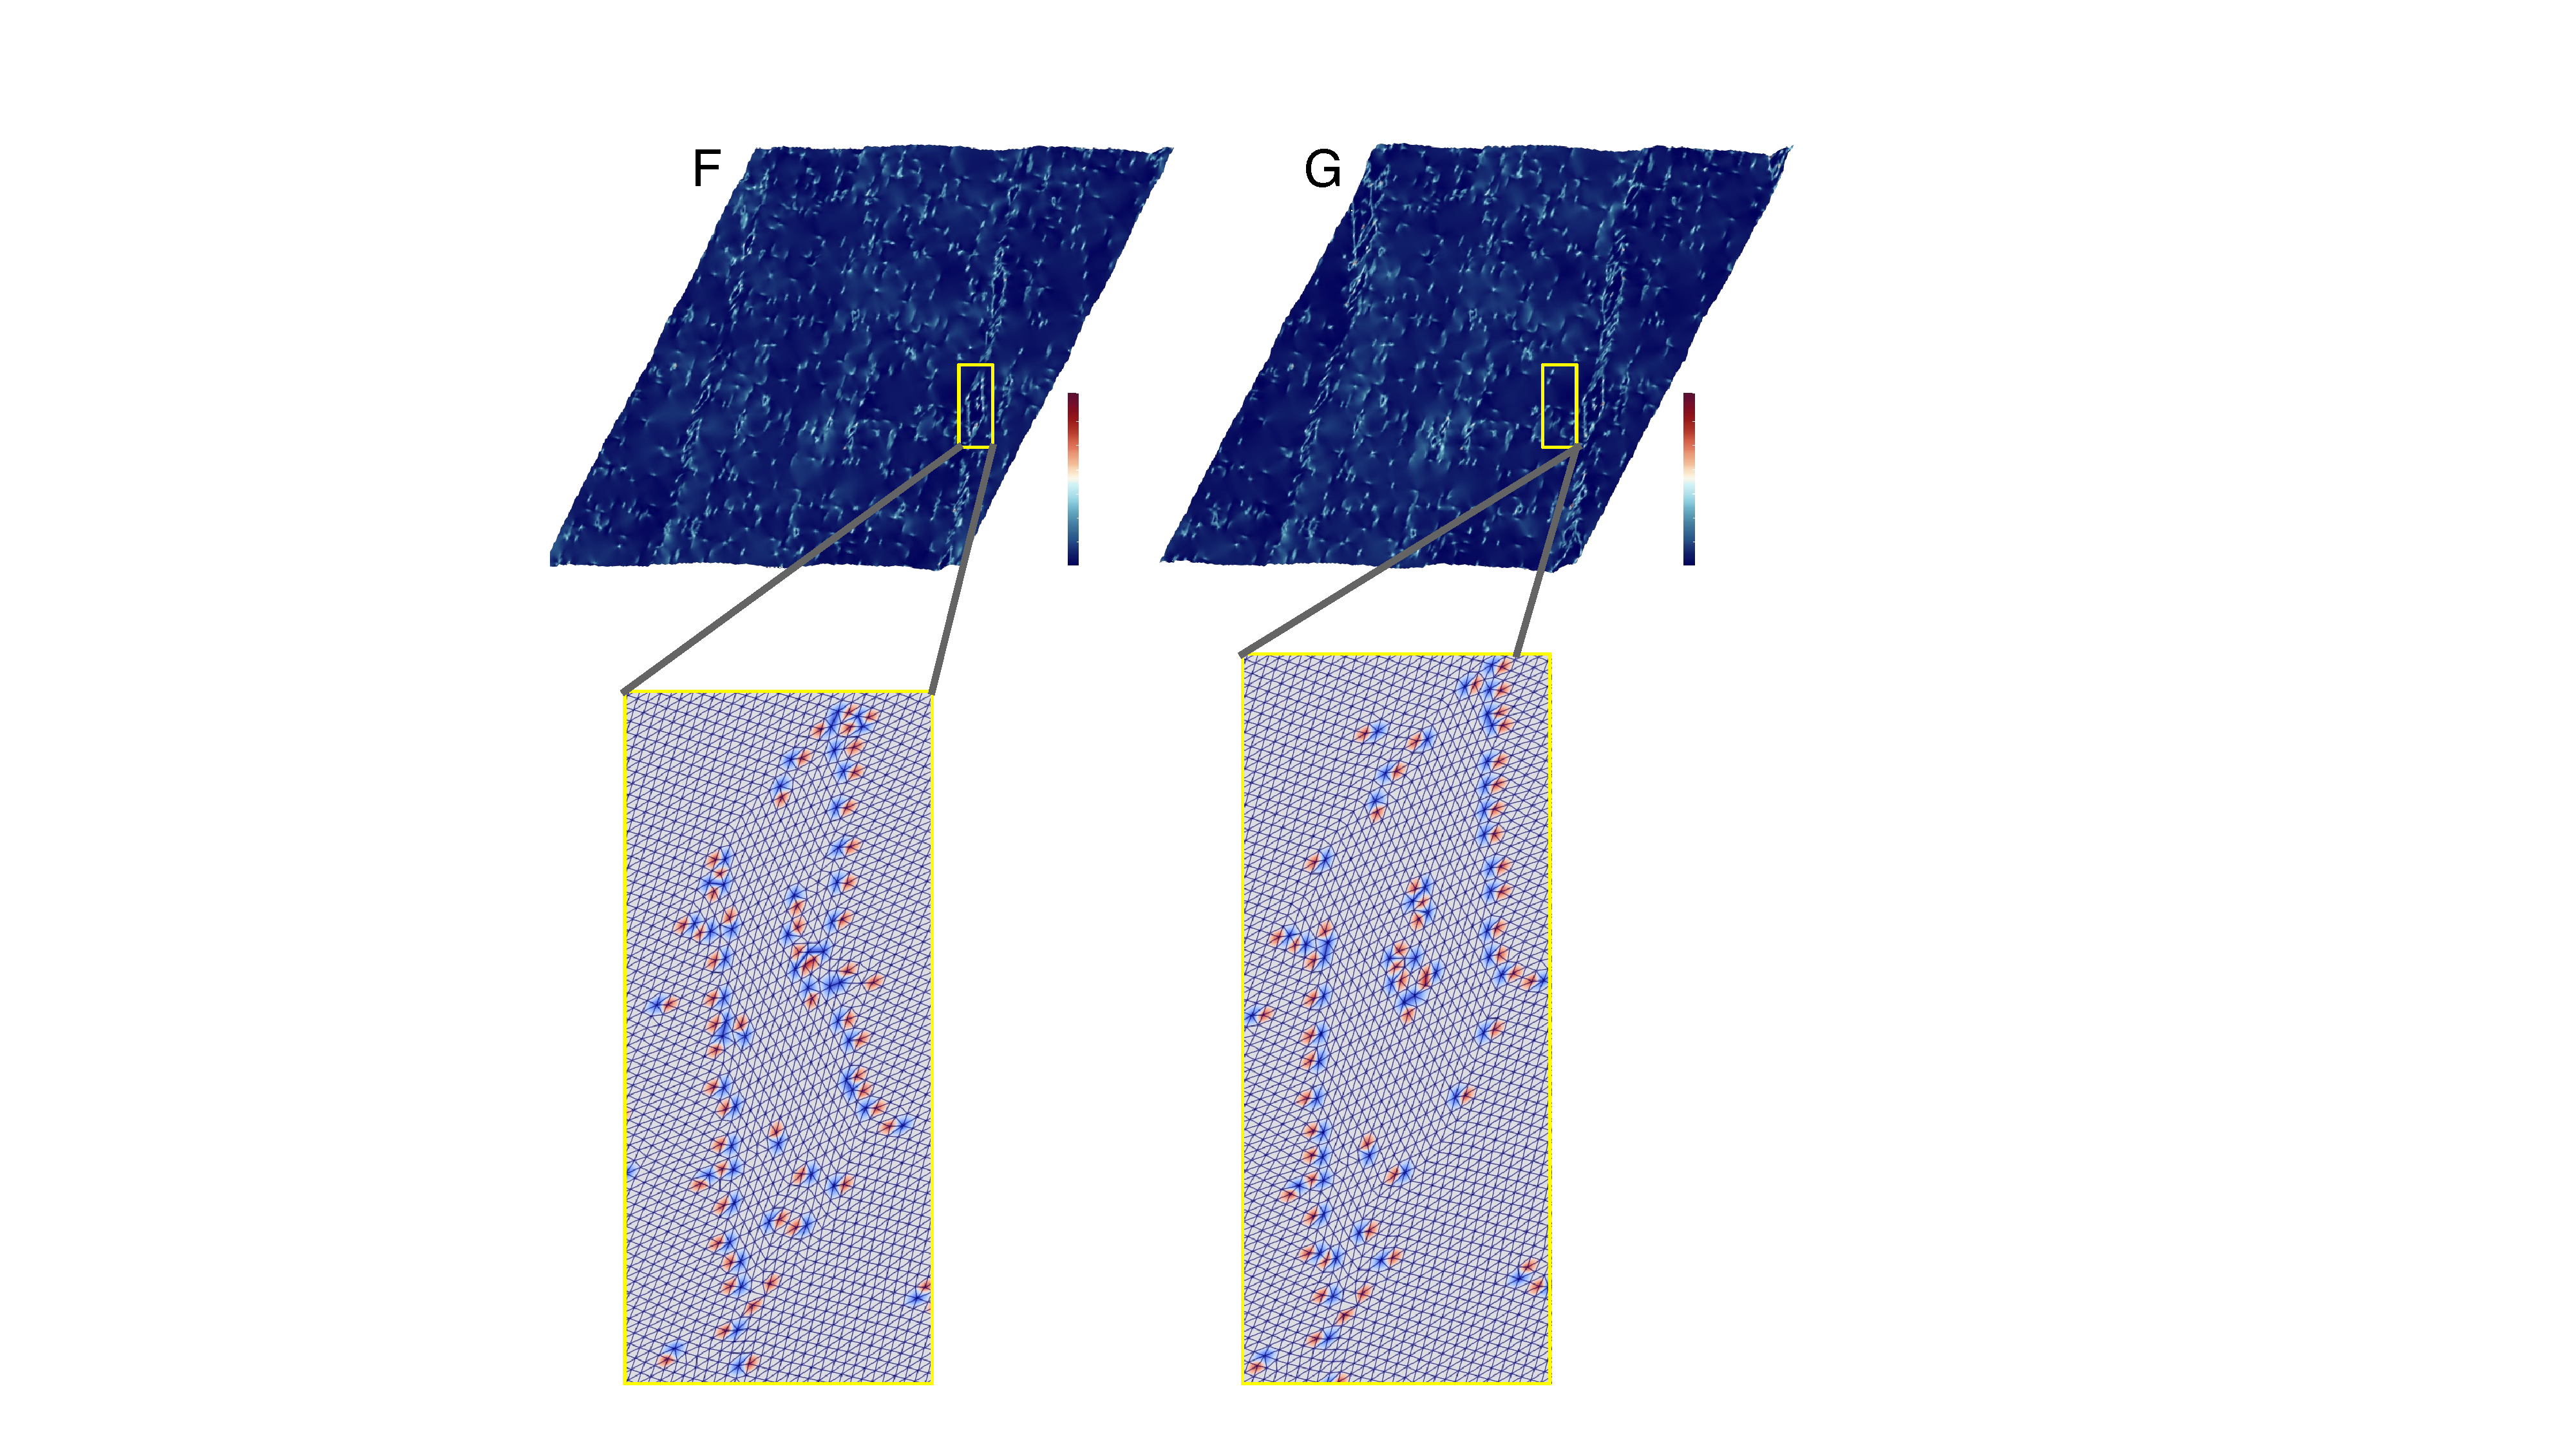
\includegraphics[scale=.35]{figures_ordering/figure_13.pdf}
\caption{(\textbf{Correct the location of the yellow box in (b)}) Evolution of stress fields ( \textbf{which one? which component?} ) and the associated changes in the dislocation structures during the transition  between the states $F$ and $G$.  Yellow rectangles show  the microstructural evolution of the same set of nodes. We use here  Delaunay triangulation, with 5/7 coordination defect pairs indicating dislocation positions. The formation of grain boundaries at the (second) yield point   is followed by the their propagation  in the process of the elongation of a crystal grain with fixed misorientation. Different grains appear to be  self-organizing into a system spanning shear band.}
\label{fig:3}
\end{figure}

 Our Fig. \ref{fig:3}, presenting  the snapshots of the strain-energy density field  in the states  $F$ and $G$,  illustrates in more detail the first stage of this critical transition.   Here again the  regions with higher energy  are  localized around dislocation cores. To reveal the underlying microstructural mechanism, responsible for the macroscopic stress drop, we  visualized Delaunay triangulation in selected regions which are   highlighted by yellow rectangles;  as we have already mentioned,  this  allows one  to track  through  the coordination number anomalies  the evolution of   dislocation configuration. 
 
According to the collected information,   the yield point (state $F$)  marks  the initial formation of grain boundaries which emerge as a result of  self-organization among  a large number of dislocations. Such self organization becomes possible due to the presence of both, long range elastic interactions and short range interactions induced by dislocation cores. The implied incipient development of the grain texture  marks the initial shift from   'local' to 'global'  dislocational arrangements. During  the subsequent gradual unfolding of the system spanning dislocational avalanche, exemplified by the state $G$,  the microstructural evolution is dominated by the propagation and growth of the previously created  grain boundaries. Finally,  an even more radical rearrangement of the dislocational structure,  bringing about the state $H$,   marks the  coalescence of different grains and points towards  the formation of  at least one extended shear band. 
 \begin{figure}[h!]
\includegraphics[scale=.4]{figures_ordering/figure_14.pdf}
\caption{The post-(second) yield configuration corresponding to state $H$ is presented through   the corresponding stress field.  Multi-grain texture can be  seen behind the  system spanning shear bands.}
\label{grains3}
\end{figure}
One can view  the emerging bands as representing  collections of differently oriented  grains. The corresponding mis-orientations  are controlled by the overall compatibility of the deformation field. In particular, the  ubiquitous presence  in such patterns of  low energy $\Sigma 5$  grain boundaries is  discussed in detail in \cite{Baggio2023-qu}, see also \cite{Sutton1984-us,Priester2012-wx,Randle2024-tf}.

The emerging low energy grain  boundaries are  still dislocation-rich  which  explains the necessity to nucleate a large amount of dislocations during the transition from state $G$ to state $H$. Such dislocational arrangements are   highly optimized  which suggests that at this stage of the deformation history the  self-organization becomes  global.  

We show in  Fig. \ref{grains3} a representative snapshot of the micro-configuration of the crystal in state $H$. It reveals  that the  avalanche  $G \to H$ involves both,  a  growth of an  existing  grain and  its    merger which  another grain.  This  consolidates the structure of the shear band which may be also viewed as an element  of a polycrystaline texture.  The corresponding catastrophic stress drop  may  be explained by the fact that, in view of their highly optimized nature, stresses  required to move grain boundaries are smaller  than those sufficient to move individual dislocations. 

We reiterate that  we interpret the progression  $F \to G \to H$ as the transition from quasi-elastic, pre-yield  behavior of an 'amorphopus crystal' to the actual plastic yield. We stress again that  it is  highly reminiscent of  brittle yielding in  well-annealed glasses.  The analogy is, of course,  incomplete since, for instance,  in the case of glasses the dislocational interpretation of a  structure of the shear band  would be   inappropriate.

 
\begin{figure}[h!]
\includegraphics[scale=.4]{figures_ordering/figure_15.pdf}
\caption{ Mature shear bands in the regime of stationary post-(second) yield plastic flow represented by the state $I$. Colors indicate the levels of energy density (correct?).
}
\label{fig:04}
\end{figure}






The post-yield fully plastic yielding, represented by the states $H$ abnd $I$,  can be interpreted as quasi-stationary non-equilibrium steady state  due to relative stabilization of the average stress level. A representative snapshot of the micro-configuration of the crystal in state $I$ is shown in  Fig. \ref{fig:04}. The   intermittent avalanches,  characterizing this regime,  represent the subsequent broadening and development of  the polycrystalline grain texture.  While bigger grains  occasionally merge to form larger rotated patches,  small grains continue to nucleate which requires an  increase of the number of dislocations. In this way the self-organization of dislocations within the existing shear bands continues while the latter keep  widening. Overall, despite the increase in the  number of dislocation, we observe  continuous maturation of what appears to be  a scale free hierarchical  structure while  the average macroscopic stress remains constant.
\begin{figure}[h!]
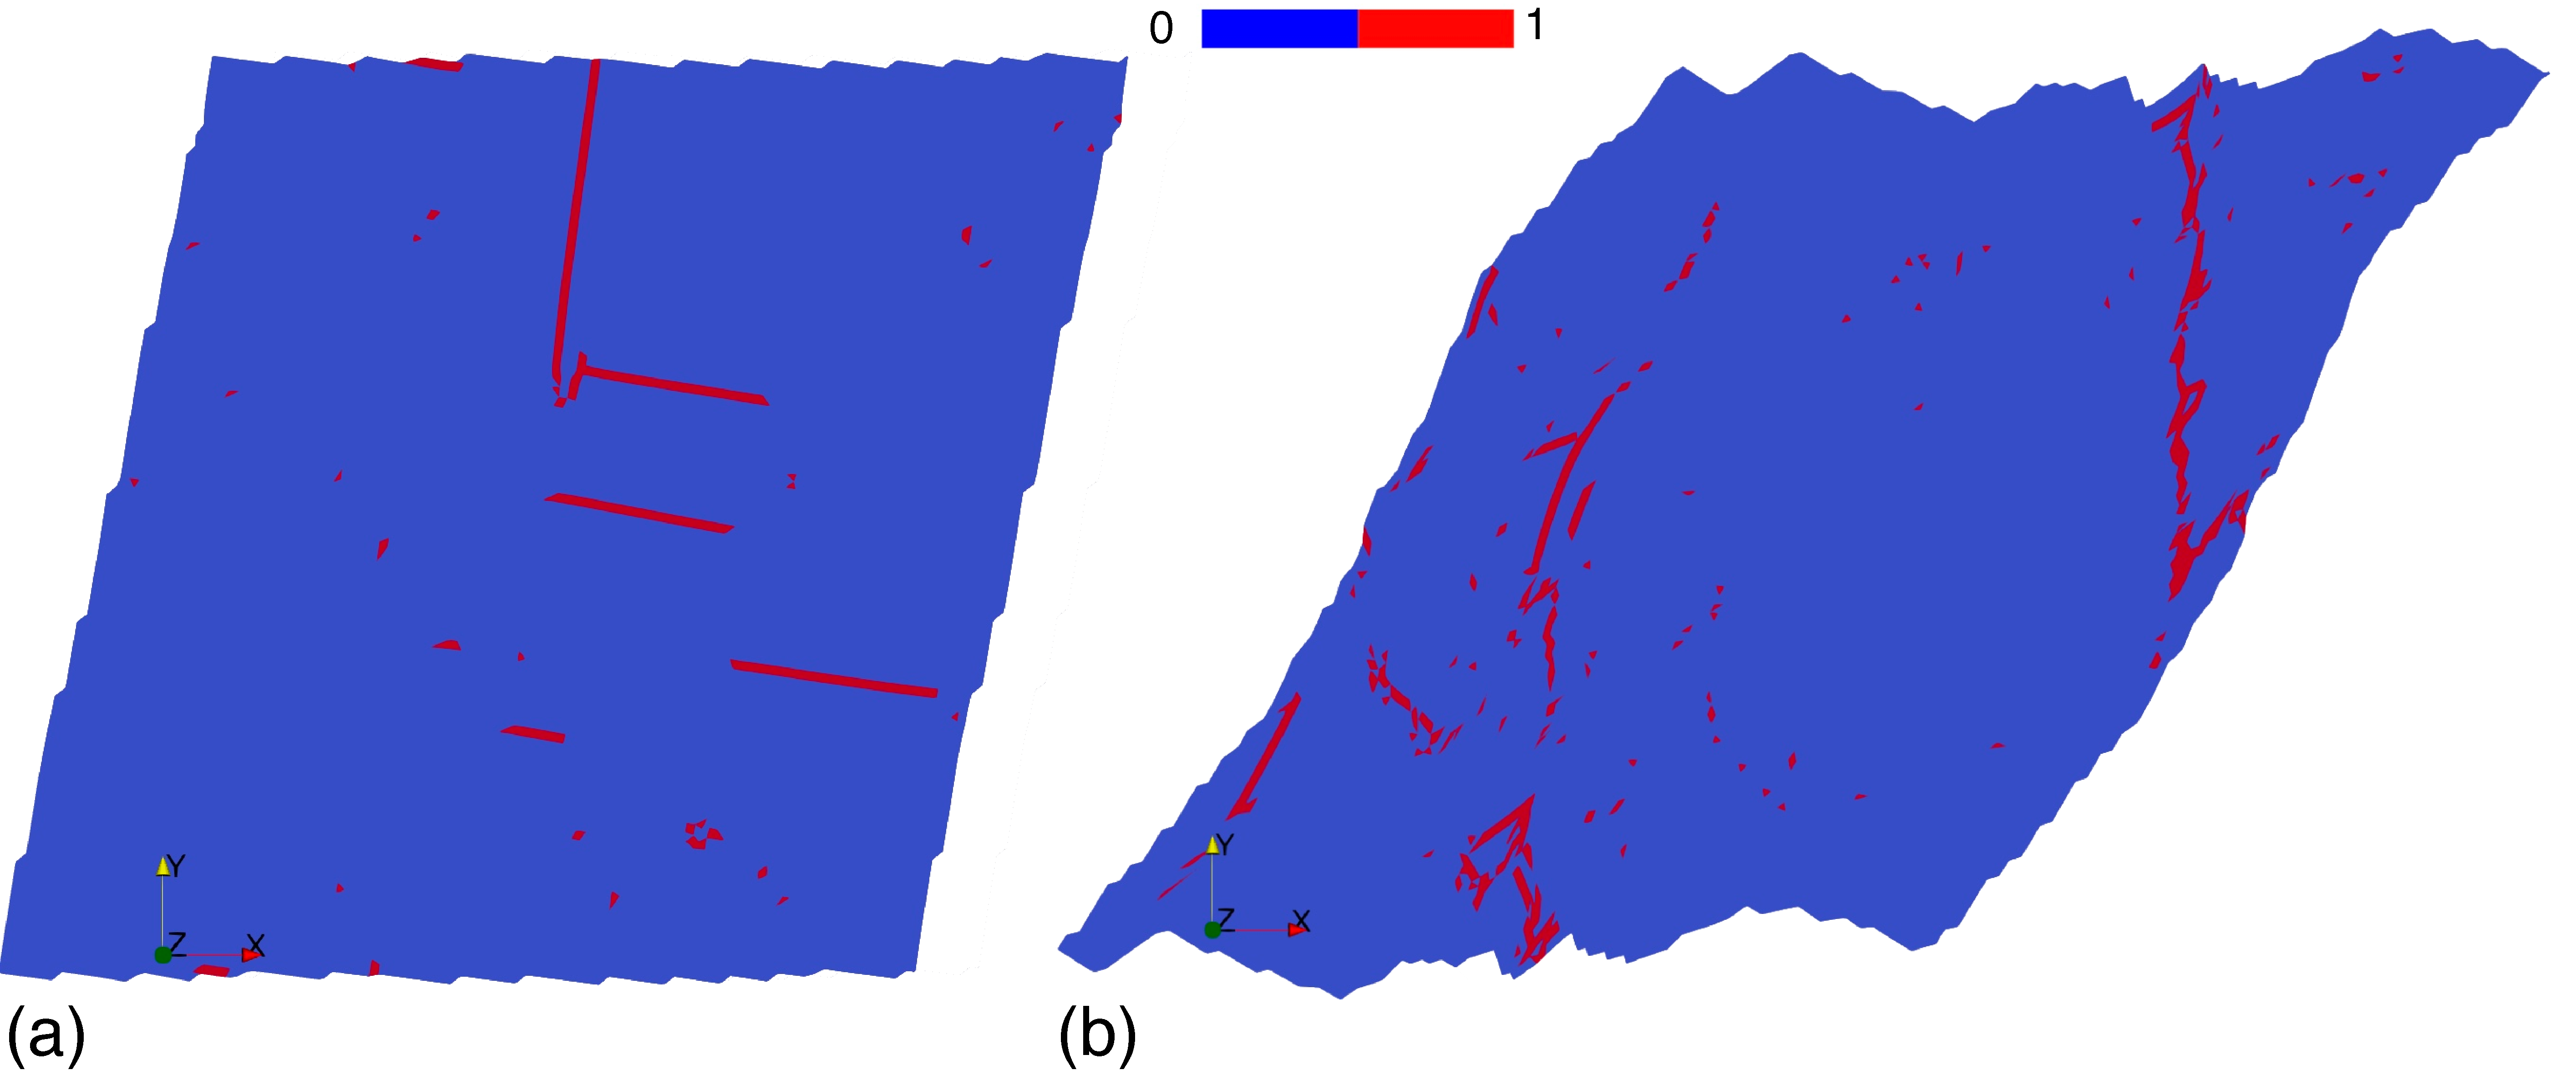
\includegraphics[scale=.1]{figures_ordering/figure_16.pdf}
\caption{The configuration of plastically activated  regions (shown in red) associated with typical stress drops: (a)   pre-(second) yield avalanche ;  (b)  post-(second) yield avalanche.}
\label{fig:plastification}
\end{figure}


 As the system transitions from isolated dislocation motion to collective dislocational behavior, it  gains access to a much broader repertoire of large-scale relaxation mechanisms, in particular, the ones that can release greater amounts of energy in a single avalanche event.  The transition from pre-yield to post-yield behavior can be then interpreted as a result  internal optimization allowing the system to cope with the necessity to dissipate larger amount of energy.  To illustrate the fundamental difference in the energy dissipation mechanisms  before (states $D$, $E$ and $F$) and after (states $H$ and $I$) the yielding transition,  we show in  Fig. \ref{fig:plastification} the typical spatial distributions of slipped regions during a single avalanche event for  both pre- and post yielding regimes. 

Using the language of amorphous plasticity, one  can say that  in the   pre-yield regime, see Fig. \ref{fig:plastification}(a), plastification occurs primarily in isolated, linear arrangements of transformed elements  showing minimal branching. These structures correspond to individual dislocations advancing  along one of the two  crystallographic planes. In this case   the energy dissipation is highly localized  while the   slip pattern is   sparse, reflecting a weak nature of dislocation interaction.  

The configuration of a typical post-yield avalanche  reveals a   different pattern of zones of plastic activity, see  Fig. \ref{fig:plastification}(b). Here, we observe   extended plastified regions showing complex branching. These structures emerge as a result of  the correlated nucleation and migration of grain boundaries producing a   texture of  almost unloaded   purely   crystalline patches which differ only by their orientation.  These observations confirm  that  in the post-yield regime the necessity  of efficient energy dissipation  indeed enforces  a  much more elaborate  spatial  structuring.
 As we have already mentioned, the implied  complexity is achieved as a result of  the transition from individual dislocation motion to their collective self-organization. 


\section{Statistic of avalanches}


We finally turn to the analysis of statistics of plastic avalanches s in our numerical experiments. Fluctuational activity  has  been lately realized as representing an important part of the mechanical  response of crystals undergoing plastic deformation \cite{Papanikolaou2017-ld,Weiss2015-eh,Zaiser2006-gk,Tarp2014-ro,Miguel2006-wd,Alava2014,Sethna2017}. Our analysis will concern   pristine crystals, but only after they have already undergone the  initial elastic instability transforming them into 'amorphous crystals'.  As we have seen,  after such a 'preparation' an initially   stable system is  effectively quenched in  apparently marginally stable  state.  In other words, we focus on what we call the 'second'  plastic yield.  The goal is to investigate the nature of plastic fluctuations by computing  the probability distribution of the energy drops associated with individual  avalanches in  pre-(second)yield regime ($\alpha<\alpha_c$) and post-(second)yield regime  ($\alpha>\alpha_c$) .  

%In both of these regimes,  separated by a system size restructuring event, plastic  flow proceeds through local instabilities  that can self organize producing a succession of broadly distributed  stress drops, each  representing an individual avalanche. As we have seen,  these events  represent  sudden, collective movements of a large number of elastically interacting dislocations.  


%We recall that in this  setting  one can distinguish between pre-(second)yield   (within  the range of strains $\alpha<\alpha_c$) and post-(second)yield (within  the range of strains $\alpha>\alpha_c$) regimes of plastic deformation. 


Before we report our results,  it is appropriate to mention again that in amorphous solids the statistics of similar energy drops has been found to be represented by a power law with a cut-off that depends on system size \cite{Tyukodi2016-dv,Budrikis2017-ex,Lerner2018-ue,Ozawa2022-xb}.  We also recall that in the context of amorphous plasticity such  behavior is usually  described in terms of simple elasto-plastic models, in which   linear elastic finite elements  can yield above some critical stress and then  trigger the yield of nearby elements as   the stress is transmitted  through the system by an elastic propagator \cite{Nicolas2018-iy,PhysRevLett.129.228002,Ferrero2019-rx,Fernandez-Castellanos2021-yn}. We reiterate that  the MTM  approach to crystal plasticity operates within  very similar finite element setting. However, there are also some important differences. Thus, phenomenological  yield thresholds are replaced by elastic instabilities in a given energy landscape and  fixed elastic propagators are replaced by the solution of a nonlinear elasticity problem. It is also important  the MTM approach to deformation is geometrically exact which allows one to  handle adequately finite rotations and elastic compatibility.

Despite these differences, our analysis  shows  that in both pre- and post-yield phases the statistics of  intermittent energy-dissipating  events  accompanying plastic
deformation  closely resembles the behavior of similar characteristics in well-annealed glasses. Specifically, we found that the probability density of energy drops  in our numerical experiments can be   well approximated by the power-law distribution with an exponential cutoff   
\begin{equation}
P(x)  \sim  x^{-\epsilon}e^{\lambda x},
\end{equation}
is exactly the result obtained in the studies of  plasticity in amorphous solids  \cite{Papanikolaou2017-ld,Weiss2021-tt,Sethna2001,Ispanovity2014-ra,Alava2014,Lehtinen2016-qy}.
\begin{figure}[h!]
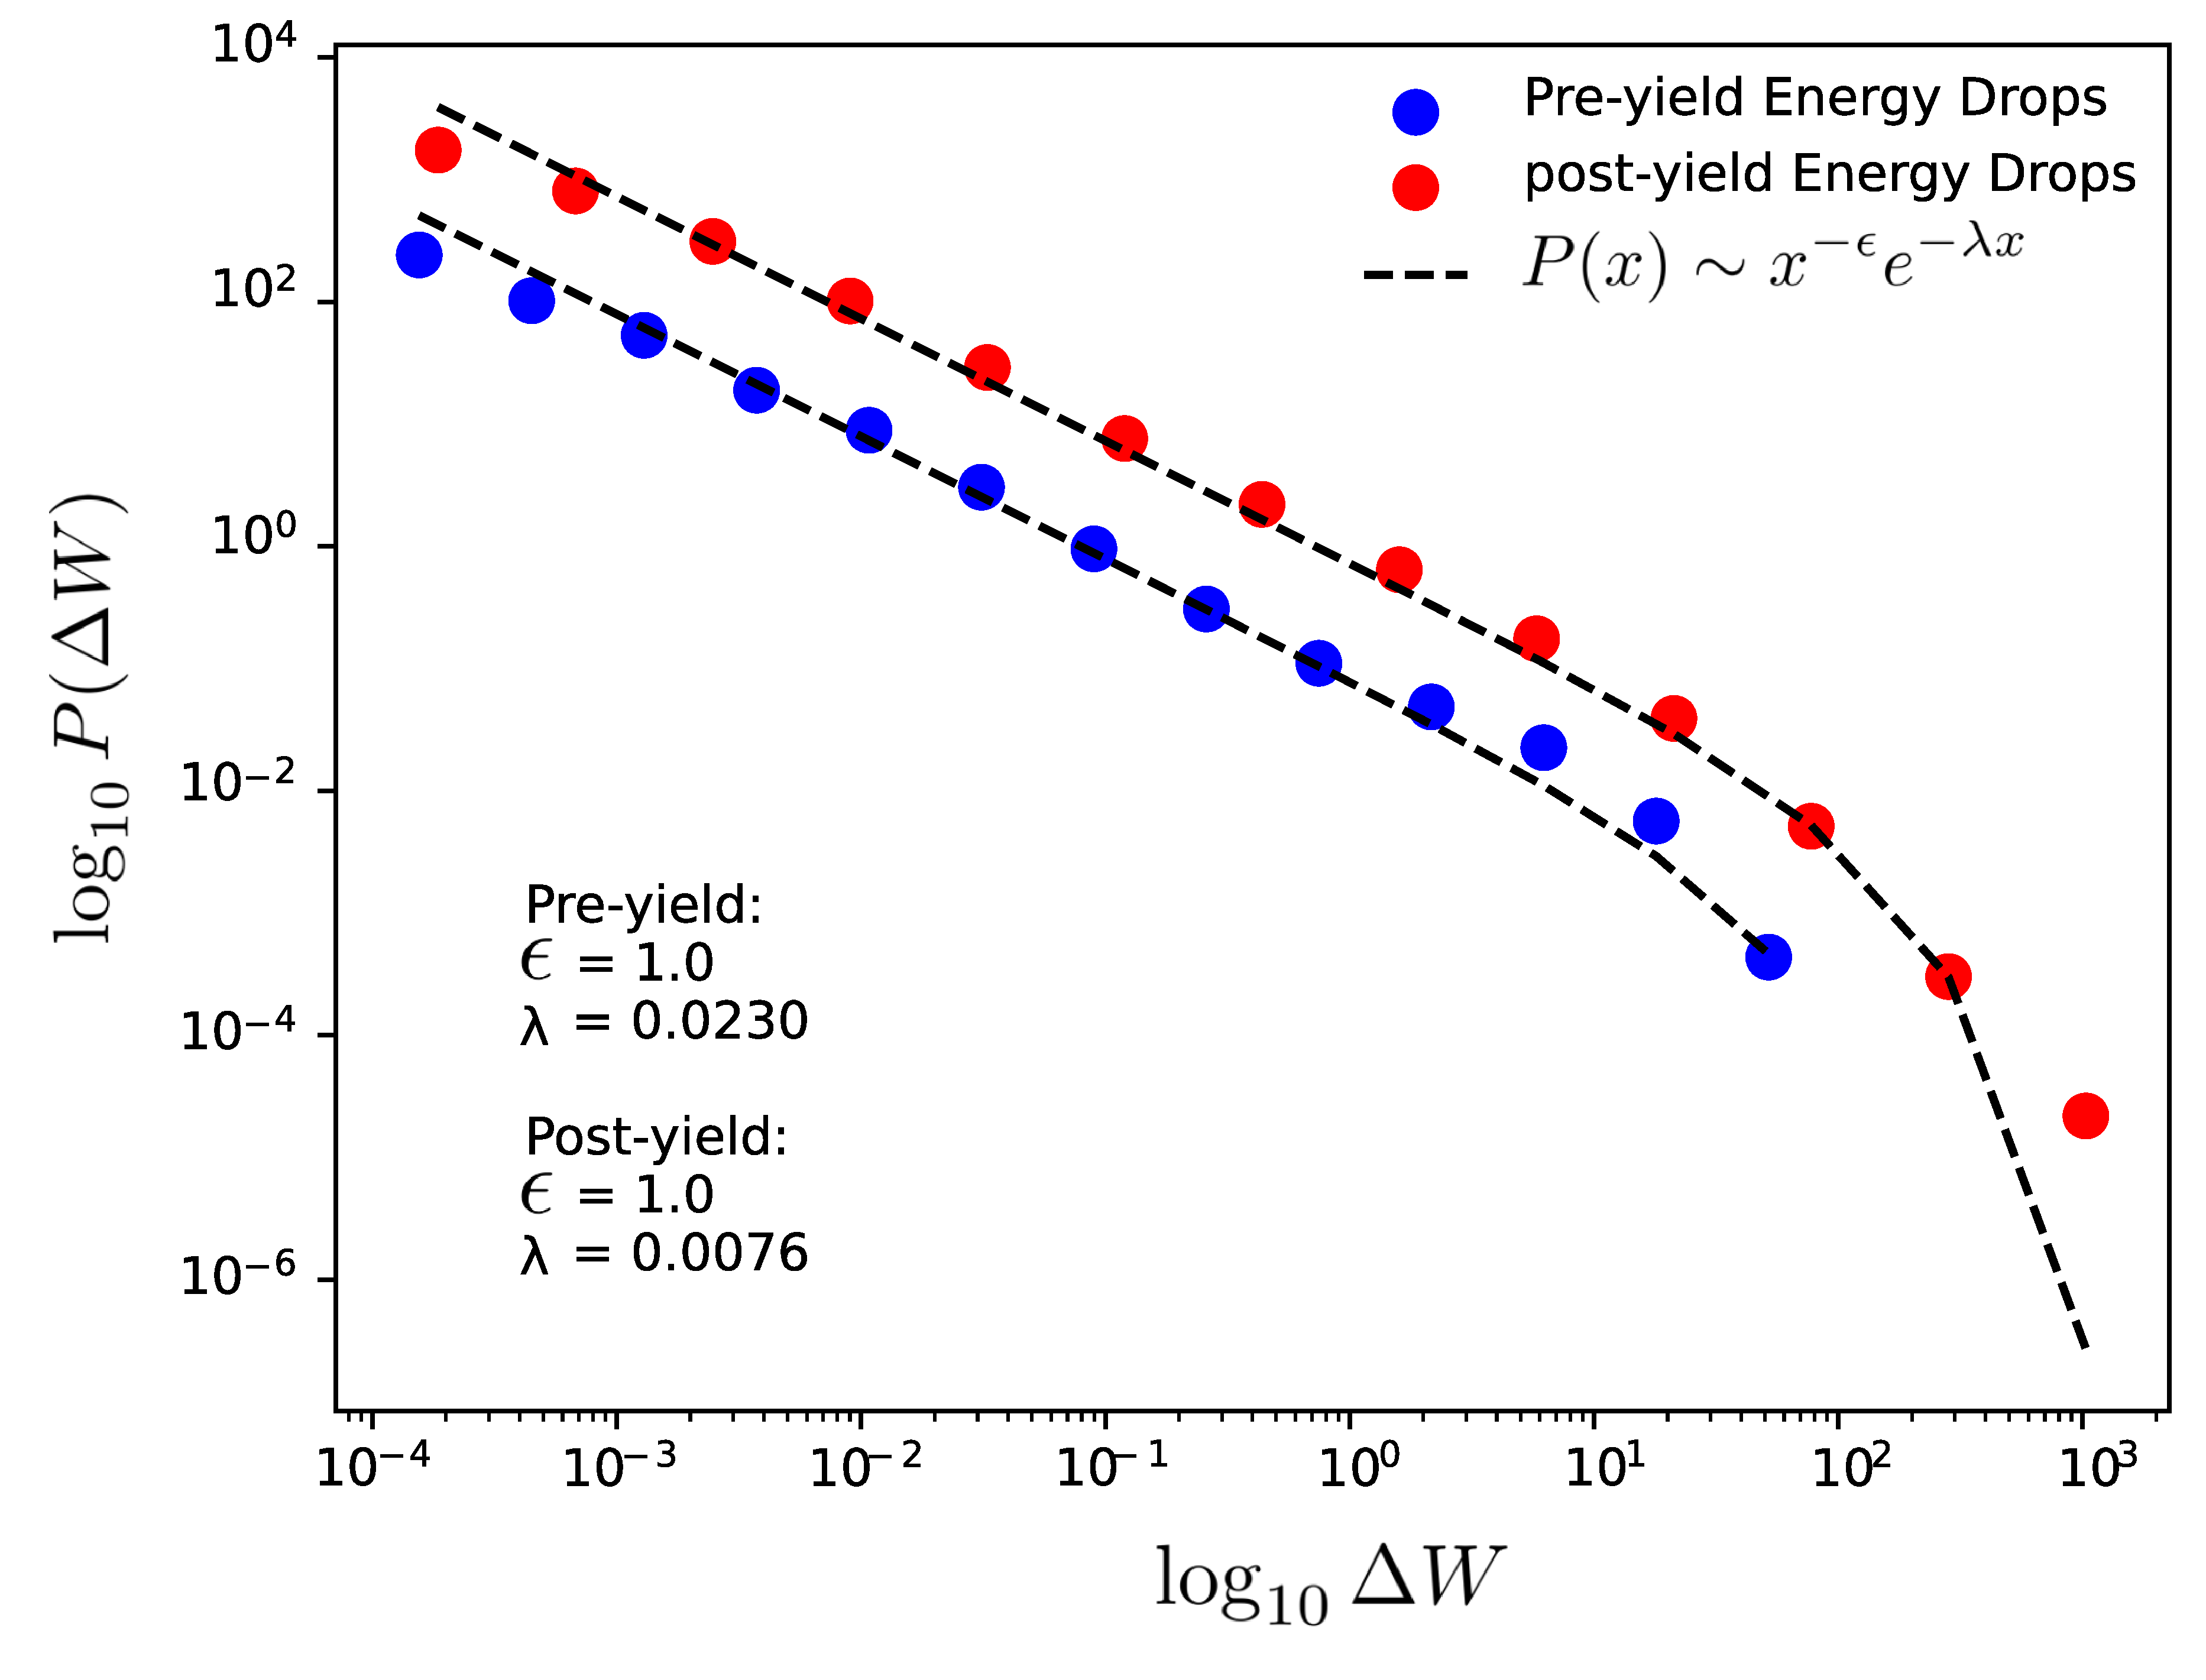
\includegraphics[scale=.11]{figures_ordering/figure_17.pdf}
\caption{Probability distribution of energy drops ($\Delta W$) during avalanches in pre-( second) yield regime (blue points) and post-(second) yield regime (red points). Both distributions are well aprroximated by a power-law with exponential cutoff.  The power law exponents $\epsilon$ in both regimes are identical. Instead the  cutoff parameters  $\lambda$  are drastically different. }\label{fig:energy_drops}
\end{figure}

Our own results are summarized  in Fig. \ref{fig:energy_drops} where we compare the statistics of  both pre- and post-(second)yield  avalanches.  One can see  that in both cases the power law range is very stable extending over up to six decades. Remarkably, despite all the dramatic differences in the macroscopic behavior, both pre-yield and post-yield energy distributions share the same power-law exponent: $\epsilon = 1.0$. This is an indication that  the  scaling behavior  remains basically unchanged across the  yielding transition despite the fact that we observe  hardening in the pre-yield regime where the dislocation number remains basically unchanged and stationary plastic flow in the post-yield regime,  where hardening disappears but  the dislocation number continuously increases. 
 The invariance of $\epsilon$ across the yielding transition  suggests that while the spatial organization of plastic events changes drastically as a result of   yielding transition from local and non-cooperative to global and collective, the statistical distribution of   events in the critical regime  remains insensitive to these microscopic details revealing a bigger picture of the global  organization of the underlying energy landscape \cite{Shang2020,oyama2021-rf}.
The universality of the obtained result is corroborated by similar findings using a completely different choice for the $GL(2, \mathbb{Z})$ energy density function \cite{perchikov2024}.


The value of the power-law exponent $\epsilon = 1.0$ has been encountered in the studies of crystal plasticity even if in somewhat  different contexts. Thus, it was found to be  a signature of an archetypically ‘‘wild’’ crystal plasticity in the sense of   \cite{Weiss2015-eh}.

An almost the same value of the power-law exponent $\epsilon = 1.0$  was obtained in discrete dislocation dynamics (DDD) studies.  In their numerical experiments conducted on disorder-free 2D samples containing a fixed number of preexisting dislocations the authors associated exactly  this value of the power-law exponent with extended  range of steady plastic flow \cite{Ispanovity2014-ra,PhysRevMaterials.5.073601}. The exponent $\epsilon = 1.0$  was also recorded in numerical experiments involving pristine crystals conducted using the scalar version of the MTM .\cite{Zhang2020-ax}. Overall,  in the literature on crystal plasticity the exponent $\epsilon = 1.0$  has been previously  linked with either dislocation jamming or self-induced glassiness  \cite{Ovaska2015-yb,Lehtinen2016-qy,Zhang2016-gh,Ruscher2019-us}.

Some  theoretical understanding of  the relation between the emergence of the power law exponent value $\epsilon = 1.0$ and the structure of the underlying energy  landscapes has been  obtained  in the case of  spin glasses. Thus,  it was shown  
that the hierarchical (ultrametric) organization of energy wells in the phase space results in an intermittent , scale-free response to quasistatic deformation \cite{Franz2017-fa,Muller2015,Berthier2019-dm,Dennis2020-jb}. Moreover, it was  shown that  in the mean-field limit the   associated distribution of  the dissipated energy  must necessarily follow power law with exponent  exactly  equal to $\epsilon = 1.0$.  It was also understood that the reason behind  this value of the exponent  is the  marginal stability of the system  \cite{Franz2017-fa,Pazmandi1999-lb,Le-Doussal2012-kv}. Note that the same arguments have been used to rationalize the observation  of  the same exponent $\epsilon = 1.0$ in numerical studies of quasi-elastic flow of structural glasses (Tyukodi et al., 2019; Ferrero and Jagla, 2019; Shang et al., 2020)~\cite{tyukodi2019avalanches,Ferrero2019-rx,Shang2020}.

We recall that  marginality of structural glasses is usually linked to the fact that they emerge  when liquid  is brought exactly to its  quenching threshold.  Similar type of marginality is also exhibited by  jammed states of granular matter that are also expected  to be at the threshold between liquid and solid behavior. In both cases  'rigidity'  results from  the fact that  dynamics has just subsided which explains why the ensuing stability is only marginal. In such states the closeness to unstable   modes makes the mechanical response   inherently intermittent, effectively mixing dynamics and statics. In the same  spirit, the recovery of  the exponent $\epsilon = 1.0$ in our numerical experiments may be suggesting that our 'amorphous crystal' is posited exactly at the threshold of mechanical stability. This is, in fact, not surprising  since the stabilization in the 'amorphous crystal' state was achieved exactly at the end of the first system-size avalanche.  Apparently, the associated  fast time dynamics  brought into the system  exactly the   level of self-generated  disorder needed  to transform  a stable (elastic) state into a marginally stable (glassy) state. Since we observe the same value of exponent $\epsilon = 1.0$ in both pre- and post-yield regimes, the achieved marginality is not even affected by the catastrophic  yielding event. This may mean that   the brittle  yielding transition does not compromise   the global organization of the emerged energy landscape while obviously  affecting the reachability of its different subdomains.



%our  pristine crystal  exactly into marginally stable configuration.  In other words, the crystal self-generated 
%
%can be considered  as an indicator of the fact that in the course of self-organization of the system it has posited itself at the threshold of mechanical stability.  Based on this understanding,
%In fact the  exponent $\epsilon = 1.0$  is consistent with models of jamming transitions in amorphous materials, suggesting that glass formation  shares underlying physics with jamming phenomena. 
%
%, through either  quench or jamming, 

%This brings us back to the idea of a similarity between  the plastic response  of our 'primed' pristine crystals and some amorphous solids, in particular,  well-annealed glasses.  It is clear that   the peculiar  macroscopic behavior of plastically deforming solids is a reflection of the complex structure of the energy landscape.  It has been argued that the  necessary level of  complexity can  emerge as a result of hierarchical (ultrametric) organization of energy wells in the phase space (Müller and Wyart, 2015; Berthier et al., 2019). \cite{???}.( \textbf{add references})
%%Müller, M., Wyart, M., 2015. Marginal stability in structural, spin, and electron glasses. Annu. Rev. Condens. Matter Phys. 6, 177.
%%Berthier, L., Biroli, G., Charbonneau, P., Corwin, E.I., Franz, S., Zamponi, F., 2019. Gardner physics in amorphous solids and beyond. J. Chem. Phys. 151,
%%010901.
%  In this case, the mechanical response under athermal quasistatic loading,  can be expected to  scale-free plastic fluctuations,  which one can link directly to  the   fine structure of the energy landscape.  
%

In contrast to the exponent $\epsilon$,   the cutoff parameter $\lambda$ differs drastically  between the pre-yielding regime, where   $\lambda = 0.0230$,  and  post-yielding regime, where  $\lambda = 0.0076$, even though in both cases we deal with the same system size. The approximately three-fold decrease in $\lambda$ after yielding indicates that large energy drops become substantially more probable in the post-yield regime.  This is a clear   evidence  of  an emergent collective behavior which manifests itself in  a much broader extent of the post-yield  avalanches.  Effectively  we observe   in the post- yield regime  an evidence of a  divergence of the characteristic   length   
 \begin{equation}
l \sim 1/\lambda.
 \end{equation}
This conjecture is supported  by the observation  that  shear bands  in the post-yield regime   traverse the whole computational domain  reaching  the size of the system. This is in stark  contrast to unequivocally subextensive localized rearrangements   taking  place in the pre-yield regime. It is appropriate to evoke  here that the  divergence of the  correlation  length is one of the major indicators that the system  has  reached  a critical state.  The physical nature of the associated generic (extended) criticality  is presently actively  debated \cite{Grinstein1995-lw,Zippelius2023-ak,Charbonneau2023-oo,Oyama2023-oj,Xing2024-tz}.

Finally we mention that our results clearly indicate that the values of parameters $\epsilon$ and $\lambda$ reflect   different aspects of the self-organization processes taking place during plastic deformation.  The persistence of $\epsilon$ over the yielding transition and the variability of $\lambda$  raises important question about  the  physical nature of  the associated  quasi-abrupt emergence of complex long range correlations which ultimately  transforms  crystallinity into glassiness.\cite{Regev2017-ks,Charbonneau2014-gv,Fu2025-tl}.
\section{Conclusions}

In this paper we performed a series of numerical experiments aimed at deeper understanding of  the phenomenon of plastic yield  in highly idealized   2D crystals in the limit of zero strain rate and negligible thermal effects. To capture the intricate underlying dislocational dynamics  we used a relatively novel theoretical  and computational tool:  a mesoscopic tensorial model  (MTM) of crystal plasticity representing a conceptual trade-off between continuum  and atomic descriptions. 


The MTM is built on the fundamental assumption that mesoscale material elements are exposed to an effective globally periodic  energy landscape  accounting for lattice-invariant shears. From the perspective of such Landau-type continuum theory with an infinite number of equivalent energy wells, plastically deformed crystal emerges as a multi-phase mixture of equivalent phases. Plastic yield can then be interpreted as an escape from the reference energy well, and plastic mechanisms can be linked to low-energy valleys in the energy landscape.  Despite its conservative appearance, the MTM approach is fundamentally dissipative with  dry friction  dissipation emerging as an averaged  description of an overdamped athermal dynamics in a rugged energy landscape.  As we explain in the paper, the internal cutoff length scale is brought into the MTM by the assumption that a mesoscopic element (cluster of atoms) deforms homogeneously with inhomogeneity emerging only at supra-mesoscopic scales. 

In comparison with other mesoscopic theories, the MTM  approach has the advantage of describing in a self-consistent manner various topological changes in dislocation configurations such including  nucleation, annihilation and  interaction with obstacles, while relying only on the information about  the inter-atomic potential.  In addition to the overall description of plastic yield at the level of stress-strain relations, the MTM approach can  capture more  subtle  effects  which depend crucially on the interplay between short and long range interactions among  dislocations. An important effect of this type, which was for us of particular interest,  is the emergence of  intermittent  dislocational avalanches. 


 While it is known that quasi-brittle yielding is  a salient feature  of well-annealed glassy materials,  here we used  the  MTM approach to show that plastic yielding in model pristine crystals leads to a remarkably similar phenomenology. More specifically, our numerical experiments  revealed that plastic yielding in  somewhat  stylized ideal crystals can be represented as a two stage process. 
 
 During the first-stage-yielding massive dislocation nucleation results  in the formation of an effectively  glassy state. More precisely,  a  system size avalanche, representing  nonlinear elastic instability,  a fast time  self-oranization phenomenon  combining nucleation and   the proliferation of defects  which  effectively transform  a pristine crystal into what we call an 'amorphous crystal'.
 
We note that the emergence of such quasi-amorphous state  after a massive dislocation nucleation event is not completely surprising. Thus,  the  mechanical response of conventional poly-crystalline solids is usually qualified as isotropic and  is treated by continuum plasticity theory similar to how it treats  other amorphous solids. What we see  is that  at least some features of amorphous response may be acquired by  pristine crystals even before the polycrystaline texture develops. In other words, the necessaary level of annealed  disorder may  result from  dislocation  self-organization at   an  almost molecular level.  

The second-stage-yielding  is preceded by pseudo-elastic deformation of  a quasi-amorphous solid  associated with only minimal dislocational activity.The activity of defects  remains  localized as in the case of 'caged' rearrangements  in  amorphous solids.  This  nominally-elastic stage of plastic deformation  which is sometimes interpreted as 'micro-plasticity', ends abruptly with  a catastrophic  phenomenon closely resembling   quasi-brittle yield in well-annealed glasses.  We therefore interpret this  system spanning event  as a transition to the actual plastic yield in a pseudo-amorphous system.  The subsequent  plastic flow takes the form of intermittent development of  a grain texture  at  almost constant stress. It  involves local and global rearrangements of the dislocational structure which takes the form  of an evolving  system of  shear bands. 
 
One of our main findings is that   in both pre- and post (second) yield regimes, plastic  flow proceeds by local instabilities at the level of single elastic elements which  are organized  in   hierarchical  way due to the presence of long range  elastic interactions. This self-organization is behind   dislocational avalanches  which takes place at   constant applied strain but which result in  stress or energy drops exhibiting power law statistics. Similarly distributed energy and stress drops  have been long known  to be a signature of  amorphous plasticity. The use of the MTM approach allowed us  to  discover that even the exponents, characterizing power law distributed avalanches,  are similar in some model systems representing amorphous and crystalline plasticity. In particular, in full agreement  to what is known about plasticity of glassy systems, here  we also found  that both pre- and post (second) yield   avalanches exhibit power law statistics with  matching exponents. This supports our idea of an 'amorphous crystal'  which is characterized by the  marginal stability of the associated defect configuration   indicative of a   hierarchical  structure of the underlying energy landscape. 
  
 
  More work would be needed to convert our initial insights, revealing various peculiar aspects of the behavior  of an over simplified prototypical system, into a deep physical  understanding of the phenomenon of plastic yield  in  realistic 3D crystals with, say  HCP, FCC and BCC symmetry.  For instance, while the developed model deals only with  quasi-statically loaded,  low dimensional  defect free model crystals at zero  temperature,  it  effectively underplays  such important physical effects of  realistic crystal plasticity  as dislocation climb, cross slip, dislocation pinning and  forest  hardening,  to mention just a few. Most importantly, only a 3D model will distinguish adequately edge, screw, and mixed dislocations, and  will be suitable to handle topologically nontrivial  dislocation entanglements. The 3D model addressing crystallographically nontrivial  crystal structures will also allow one to study the effects of the orientation of the samples in the loading device which are known to affect strongly the complexity of the emerging dislocation patterns.  To account adequately for all these important physical effects,  one would also need to quantitatively calibrate the 3D version of the MTM by a systematic comparing  with parallel MD simulations and developing a rigorous conceptual bridge between the notions used to describe atomic and mesoscopic scales. 
 
 
\emph{ Acknowledgments. } The authors thank G. Tejedor and A. Ahadi for helpful discussions. The work of O.U.S. was supported  by  the grants ANR-18-CE42-0017-03, ANR-19-CE08-0010-01, ANR-20-CE91-0010. N.G. and L. T. were supported by the grants ANR-17-CE08-0047-02, ANR–21-CE08-MESOCRYSP and ERC-H2020-MSCA-RISE-2020-101008140.

%\bibliography{plasticity.bib}
\bibliography{./formatted.bib}

\end{document}


%https://www.scirp.org/journal/paperinformation.aspx?paperid=108300
%
%https://www.scientific.net/KEM.725.636

